\documentclass[a4paper,14pt]{article}
\usepackage{blindtext}
\usepackage[T2A]{fontenc}
\usepackage[utf8]{inputenc}
\usepackage[english,russian]{babel}
\usepackage{listings}
\usepackage{geometry}
\usepackage{amssymb}
\usepackage{amsmath}
\usepackage[14pt]{extsizes}
\geometry{left=3cm}
\geometry{right=1.5cm}
\geometry{top=2cm}
\geometry{bottom=2cm}
\pagestyle{plain}
\usepackage{pgfplots}
\usepackage{filecontents}
\usepackage{graphicx}
\usepackage{indentfirst}
\DeclareGraphicsExtensions{.png}
\graphicspath{{images/}}
\usetikzlibrary{datavisualization}
\usetikzlibrary{datavisualization.formats.functions}
\usepackage{tabularx}
\pgfplotsset{width=7 cm}
\usepackage{xcolor}
%\renewcommand{\rmdefault}{ftm}
%\usepackage{mathptmx}
\usepackage{setspace}
% \usepackage{minted}

%\полуторный интервал
\onehalfspacing
\frenchspacing

\usepackage{tocloft}
\frenchspacing
\setcounter{page}{2}
\usepackage{multirow}
\usepackage{float}
\usepackage{multirow}

\renewcommand{\cftsecdotsep}{\cftdot}
\renewcommand{\cftsecleader}{\cftdotfill{\cftsecdotsep}}
\renewcommand{\cftsubsecleader}{\cftdotfill{\cftsecdotsep}}
\renewcommand{\cftsubsubsecleader}{\cftdotfill{\cftsecdotsep}}

%\renewcommand\cftchapdotsep{\cftdot}
%\renewcommand\cftsecdotsep{\cftdot}
%\renewcommand{\cftchapleader}{\cftdotfill{\cftchapdotsep}}

% Для измененных титулов глав:
% % подключаем нужные пакеты
%\definecolor{gray75}{gray}{0.75} % определяем цвет
%\newcommand{\hsp}{\hspace{20pt}} % длина линии в 20pt
% titleformat определяет стиль
%\titleformat{\chapter}[hang]{\Huge\bfseries}{\thechapter\hsp\textcolor{black}{|}\hsp}{0pt}{\Huge\bfseries}
%\usepackage{titlesec, blindtext, color}
%\titleformat{\chapter}[hang]{\Huge\bfseries}{\thechapter\hsp\textcolor{black}{|}\hsp}{0pt}{\Huge\bfseries}


\begin{document}
%\pgfplotsset{compat=1.17}

\textbf{1. Понятие модели и моделирования. Общая классификация моделей. Требования к моделям. Примеры из конкретных предметных областей.}

\textbf{Моделирование} -- это методология разработки и изучения объекта, основанная на замене этого
объекта моделью и работе в дальнейшем с этой моделью.

\textbf{Объект} -- система, процесс, явление, материальная или нематериальная сущность.

\textbf{Модель} -- представление объекта в виде, отличном от облика или формы его реального существования или функционирования.
Модель в процессе изучения замещает объект-оригинал, сохраняя некоторые важные для данного исследования типичные его черты.

\textbf{Классификация моделей:}
\begin{itemize}
	\item натурные (материальные) -- физические, геометрические, аналоговые;
	\item абстрактные (нематериальные) -- символьные (графические, текстовые, математические), интуитивные, модели суждения;
\end{itemize}

\begin{figure}[!h]
	\center{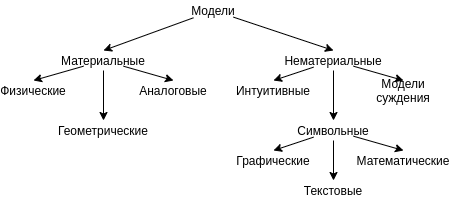
\includegraphics[width=16cm]{klassifik}}
	%\caption{График зависимости $T(x)$ при $F_0 = 0$ (шаш 0.0001).}
	\label{fig:klassifik}
\end{figure}

\textbf{Геометрические модели} -- макеты.

\textbf{Физические модели} -- воспроизводят реальные условия функционирования объектов
(например, модель самолета в аэротрубе).

\textbf{Аналоговые модели} -- один процесс заменяется другим (например, существует процесс передачи тепла.
Диффузия заменяется протеканием электрического тока. Строится электрическая цепь
и определяются потоки тепла).

\textbf{Модели суждения} -- мировоззрение.

\textbf{Интуитивные модели} -- например, в мозге протекают процессы, прогнозирующие исход
дорожной ситуации, когда хотим перейти дорогу.

\textbf{Графические модели} -- рисунки, диаграммы, чертежи.

\textbf{Текстовые модели} -- программы.

\textbf{Математическая модель} -- представление объекта в виде уравнений, логических соотношений, формул.

\textbf{Математическое моделирование} -- методология, основанная на замене объекта
математической моделью и исследовании этой модели.

\textbf{Требования к модели:}

\begin{itemize}
	\item адекватность -- соответствие объекту и предъявленным требованиям;
	\item универсальность;
	\item точность -- удовлетворение требований к погрешности результата;
	\item экономичность -- соответствие цена - качество.
\end{itemize}

\textbf{Предметные области}, в которых применяется математическое моделирование:

\begin{itemize}
	\item прогнозирование событий;
	\item исследование объектов, которые при каждом своем применении уничтожаются;
	\item дорогостоящие объекты с длительным сроком разработки;
	\item отсутствие объекта-оригинала;
	\item исследование длительного по времени эволюции процесса.
\end{itemize}

\textbf{2. Схема вычислительного эксперимента.}

\begin{figure}[!h]
	\center{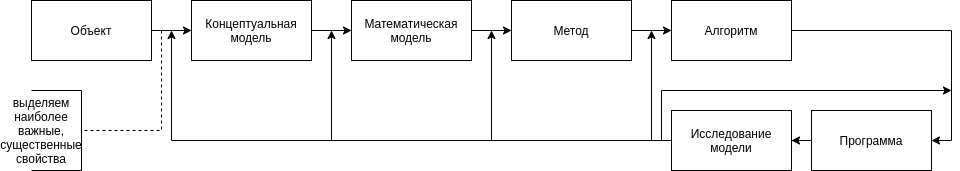
\includegraphics[width=17cm]{schema_exp}}
	%\caption{График зависимости $T(x)$ при $F_0 = 0$ (шаш 0.0001).}
	\label{fig:schema_exp}
\end{figure}

Концептуальная модель = содержательная модель = расчетная схема.

Исследование модели -- тестирование программы. В зависимости от найденных проблем
можно вернуться к одному из предедущих этапов.

Проще:

\begin{itemize}
	\item модель;
	\item алгоритм;
	\item программа.
\end{itemize}

\textbf{3. Понятие математической модели. Функции моделей. Источники погрешностей при построении модели, алгоритмизации и программировании.}

\textbf{Математическая модель} -- представление объекта в виде уравнений, логических соотношений, формул.

\textbf{Классификация математических моделей:}

\begin{itemize}
	\item имитационные (массового обслуживания);
	\item функциональные (регулярные);
	\item модели идентификации.
\end{itemize}

Имитационное моделирование применяется в тех случаях, когда необходимо
учесть возможно большее разнообразие исходных данных, изучить
протекание процессов в различных условиях.

\textbf{Функции моделей (математических).}
\begin{itemize}
	\item Описательная функция.
	
	Математическое моделирование объекта помогает понять, как устроен объект, его структуру, свойства, законы развития и взаимодействия с окружающим миром.
	
	\item Управленческая функция.
	Показывает, что заключенные в математических моделях закономерности могут помочь принять научно обоснованные решения по его совершенствованию.
	\item Выступают в роли предмета или средства исследования.
	\item Интерпретационная функция.
	
	Математическая модель может не только объяснить, но и позволяет описать множество частных случаев, которые могут быть выведены из нее логически и не требуют специального описания.
	\item Прогностическая функция.
\end{itemize}

\textbf{Функции моделей.}

\begin{itemize}
	\item Познание.
	
	Прежде чем разрабатывать модель, нужно получить
	информационное оснащение (материальные коэффициенты) расчетами или из экспериментов.
	Чем более детально описывается процесс, тем больше требуется информации.
	\item Прогнозирование (предсказание).
	
	Прогнозирование используется для оптимизации.
	\item Передача информации.
	
	При образовании систем -- передача информации между подсистемами.
	\item Применение в тренажерах.
\end{itemize}

\textbf{Источники погрешностей при вычислениях:}

\begin{itemize}
	\item погрешность модели -- несоответствие математического описания задачи
	реальной действительности;
	\item погрешность исходных данных (неустранимая);
	\item погрешность метода.
	
	Связана со способом решения поставленной математической задачи.
	\item погрешность округления.
	
	Погрешность округления обусловлена необходимостью выполнения
	арифметических операций над числами, усеченными до количества
	разрядов, зависящего от применяемой вычислительной техники.
\end{itemize}

Существует взаимная компенсация погрешностей.

\textbf{4. Понятие корректности постановки задач. Привести примеры некорректно поставленных и слабо обусловленных задач и  неустойчивых алгоритмов.}

Задача называется \textbf{корректно поставленной}, если
ее решение существует, единственно и устойчиво по входным данным.

$y = A(x)$

$A(x + \delta) = y + \delta y$

Если при $\delta x \rightarrow 0 $ $\delta y \rightarrow 0 $, то задача устойчива.

\textbf{Устойчивость по входным данным} означает, что малые изменения входных данных
должны приводить к малым изменениям результата.

Если $\delta y$ большое, то это некорректно поставленная задача.

Часто задача формально считается корректно поставленной
и устойчивой:

$\delta y = c \delta x, c = const.$

Если константа $c$ большая, то малые изменения входных данных
все равно приведут к сильному изменению результата -- 
это слабоустойчивая задача. Такая задача мало отличается
от неустойчивой.

Если $\delta x \rightarrow 0$, а $\delta y$ большое,
то это некорректно поставленная задача.

Помимо неустойчивости формулировки самой задачи, алгоритм
ее решение (алгоритм) может быть также неустойчивым.

\textbf{Пример неустойчивой задачи}

$y = \frac{d}{dt} f(t) = f'(t)$

$y = \delta y = (f(t) + \delta f)' = f'(t) + (\delta f)'$

$\delta y = (\delta f)'$

$\delta f = \frac{1}{n} sin \, n^2 \, t \rightarrow sin^2 (t + T) = sin \, n^2 \, 2 \pi (n^2 \,T =2 \pi, T = \frac{2 \pi}{^2} )$

$(\delta f)' = n \, cos^2 \, t$

При $n \rightarrow \infty, \delta f \rightarrow 0$

$\delta y \rightarrow \infty$

Можно получить даже отрицательную производную, хотя на самом деле она положительна.

\textbf{Пример}

$u'(x) = - \alpha u, \alpha > 0$

$u(x) = u_0 e ^{-\alpha x}$

\begin{figure}[!h]
	\center{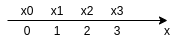
\includegraphics[width=10cm]{pr1}}
	%\caption{График зависимости $T(x)$ при $F_0 = 0$ (шаш 0.0001).}
	\label{fig:pr1}
\end{figure}
\newpage
$u(x) \rightarrow y, u(x_i) \rightarrow y_i$

$y_{n+1} = y_n + h u_n' = y_n + h (- \alpha y_n) = y_n (1 - h \alpha)$

\begin{figure}[!h]
	\center{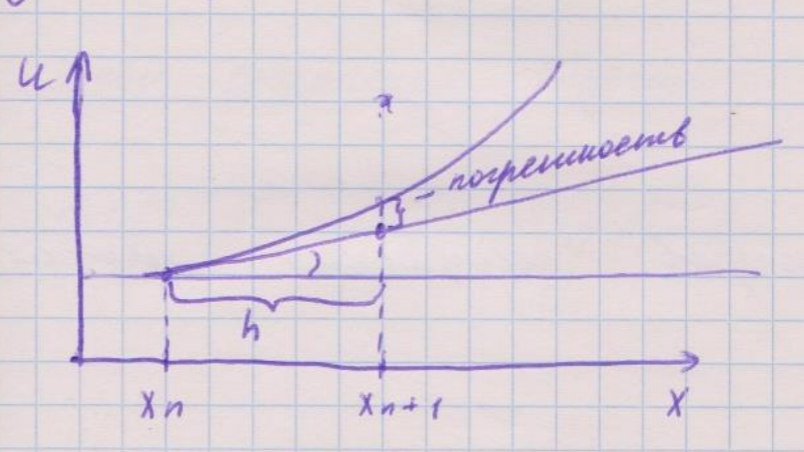
\includegraphics[width=10cm]{pr2}}
	%\caption{График зависимости $T(x)$ при $F_0 = 0$ (шаш 0.0001).}
	\label{fig:pr2}
\end{figure}

Если $(1 - \alpha) < 0$, возникают "пилообразные решения".
Чтобы этого избежать, необходимо ограничение на $h$.

$1 - h \alpha > 0 \Leftrightarrow h < \frac{1}{\alpha}.$ 

Получим относительно устойчивое решение.

\begin{figure}[!h]
	\center{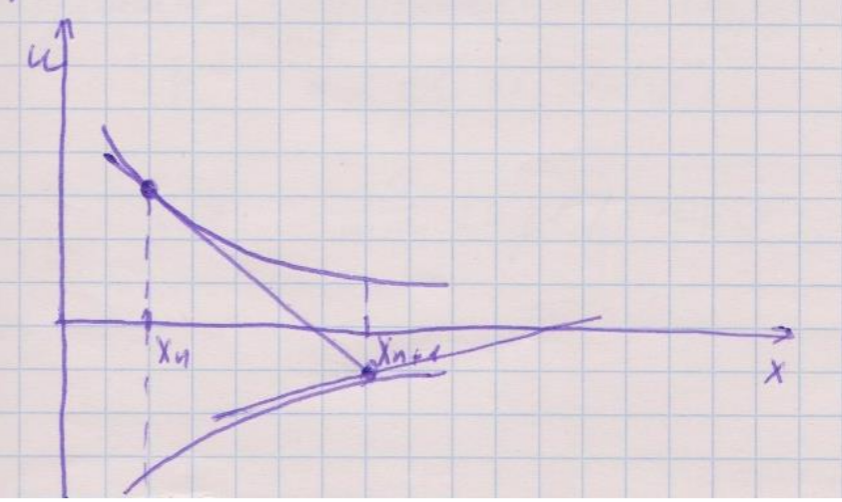
\includegraphics[width=10cm]{pr22}}
	%\caption{График зависимости $T(x)$ при $F_0 = 0$ (шаш 0.0001).}
	\label{fig:pr21}
\end{figure}

$y_{n + 1} = y_n + h u_{n+1}' = y_n + h (- \alpha y_{n+1})$

$y_{n + 1} (1 - \alpha h) = y_n$

$y_{n + 1} = \frac{y_n}{1 + \alpha h}$ -- грубое решение, но пилообразные решения
не образуются. Схема абсолютно устойчива.

\begin{figure}[!h]
	\center{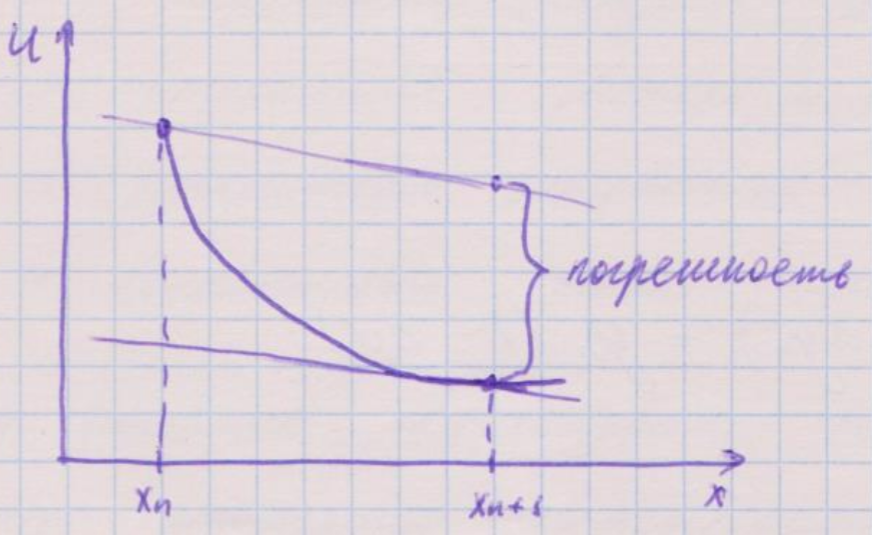
\includegraphics[width=10cm]{pr23}}
	%\caption{График зависимости $T(x)$ при $F_0 = 0$ (шаш 0.0001).}
	\label{fig:pr23}
\end{figure}

\textbf{Пример}

В качестве примера плохой обусловленности рассмотрим задачу

\begin{eqnarray}
	u'(x) = u - x, 0 \leq x \leq 100, \\
	u(0) = 1.
\end{eqnarray}


Общее решение уравнения (1) содержит одну произвольную постоянную 

$u(x, c) = 1 + x + c e^x$.

При начальном условии (2) она равна $c = 0$, так что $u(100) = 101$. 
Однако небольшое изменение начального условия $\bar{u}(0) = 1.000001$ меняет постоянную
$c = 10^{-6}$; тогда $\bar{u}(100) \approx 2.7 \cdot 10^{37}$, т. е.
решение изменилось очень сильно.

\newpage
\textbf{5. Общая классификация методов построения математических моделей.}

\textbf{Методы получения моделей:}

\begin{itemize}
	\item на основе фундаментальных законов природы;
	\item вариационные принципы (принцип Гамильтона, принцип Ферма) -- 
	система переходит из одного состояния в другое так, что некоторая связанная с ней
	величина становится экстремальной;
	\item построение иерархии моделей (снизу вверх и сверху вниз);
	\item метод аналогий.
\end{itemize}

Наиболее распространенный метод построения моделей.
Состоит в применении фундаментальных законов природы к 
конкретной ситуации. Эти законы общепризнаны, 
многократно подтверждены опытом, служат основой множества 
научно-технических достижений. Примеры таких законов: закон 
сохранения энергии, закон сохранения импульса, закон сохранения массы.

Пример: пуля врезается в брусок.

Из закона сохранения импульса получается простейшая 
математическая модель движения ракеты (в пренебрежении сопротивлением
воздуха, гравитацией).

Вариационный принцип гласит, что из всех возможных движений 
изучаемого объекта в действительности реализуется только то,
на котором некоторая связанная 
с объектом величина достигает своего экстремального значения.

При использовании вариационного принципа движение описывается 
при помощи так называемого конфигурационного пространства, 
построенного из обобщенных координат $q$, 
обобщенных скоростей $ \dot{q}$ и времени $t$. 
Основными понятиямиэтой теории, в которой движение во все 
моменты времени полностью определяется набором величин
$q(t)$и $\dot{q}(t)$, являются понятия функции Лагранжа
$L$ и действия по Гамильтону $S$.

Оптимально выбираемый уровень моделирования существенно зависит от
его целей: не обязательно использовать модель высокого уровня, 
существенно более затратную по компьютерным ресурсам, если в этом 
нетпрактической необходимости. Но и в противном случае построение 
математических моделей сразу во <<всей полноте>>, с учетом всех факторов,
существенных для его поведения, не бывает оправданным.

Более результативным оказывается подход, реализующий принцип <<от 
простого к сложному>>, когда после достаточно подробного изучения не
очень сложной модели делается следующий шаг --
отказ от одногоили нескольких упрощающих предположений, идеализирующих 
изучаемый объект. При этом возникает цепочка (иерархия) все более 
полныхмоделей, каждая из которых обобщает предыдущие, включая их 
в качестве частного случая. Путь <<от простого к сложному>> дает возможность
поэтапно изучать все более реалистичные модели и сравниватьих свойства.

Иерархия математических моделей часто строится и по противоположному
принципу <<от сложного к простому>>, <<от общего к частному>>.
В этом случае реализуется путь <<сверху вниз>> -- из достаточно
общей и сложной модели при соответствующих упрощающих предположениях 
и конкретизациях рассматриваемого объекта, определяемых протекающими 
в нем процессами, его геометрией и т. д., получается последовательность все 
более простых (но имеющих уменьшающуюсяобласть применимости) моделей.
Такой подход позволяет сразу установить некоторые общие свойства 
объекта, конкретизируя и дополняя ихв частных ситуациях. 
Длина образующейся при этом цепочки можетбыть весьма значительной.

В огромном числе случаев при попытке построить модель какого-либо 
объекта либо невозможно прямо указать законы сохранения или вариационные
принципы, которым он подчиняется, либо, с точки зрения наших сегодняшних
знаний, вообще нет уверенности в существовании подобных законов, допускающих
математическую формулировку. К таким объектам относятся, например, системы
с заметным вмешательством людей, в частности экономические системы.

Одним из плодотворных подходов к построению моделей такого рода объектов
является использование аналогий с уже изученными явлениями: методы
и результаты, разработанные и накопленные при математическом моделировании
одних явлений, переносятся <<по аналогии>> на широкие классы совсем других
процессов. Например, известны механико-экономические аналогии (использование
идеи <<насыщения>>:скорость роста со временем какой-либо величины пропорциональна
произведению текущего значения этой величины на разность между ее предельным
и текущим значениями, использование законов сохранения, переходов с микро-
на макроуровень), термодинамико-экономические аналогии (представления о 
стационарных процессах, равновесных состояниях, переход от дискретной
к непрерывной модели) и др. Применение подобных аналогий позволяет 
глубже понять принципиальныесвойства трудноформализуемых объектов.


\textbf{6. Понятие ОДУ. Сведение ОДУ произвольного порядка к системе ОДУ первого порядка. Привести примеры.}

\textbf{Дифференциальное уравнение (ДУ)} -- это уравнение, в которое входят производные (производная)
функции, которую надо найти. В ДУ могут входить сама функция, независимые переменные и параметры.

$u'(x) = x^2 + u^2$

Порядок ДУ определяется наивысшим порядком производной, входящей в него.

Порядок входящих в уравнение производных может быть различен (формально 
он ничем не ограничен). Производные, функции, независимые переменные и 
параметры могут входить в уравнение в различных комбинациях или могут 
отсутствовать вовсе, кроме хотя бы одной производной.

ДУ называется \textbf{обыковенным дифференциальным уравнением (ОДУ)}, если
функция зависит только от одной переменной.

$F(n^{(n)}, u^{(n-1)}, ..., u, x) = 0$

Обыкновенным дифференциальным уравнением можно описать задачи движения системы
взаимодействующих материальных точек, химической кинетики, электрических
цепей, сопротивления материалов (например, статический прогиб упругого стержня)
и многие другие.

ОДУ n-го порядка при помощи замены $u^{(k)}(x) \equiv u_k(x)$ можно
свести к эквивалентной системе n уравнений первого порядка.

\textbf{Сведение ОДУ n-го порядка к системе ОДУ первого порядка}

$u^{(n)} = f(x, u, u', u'', ..., u^{(n-1)})$

Вводятся новые переменные:

$u' = u_1$

$u'' = u_2$

$u^{(k)} = u_k$

Очевидно, что $u_k' = (u^{(k)})' = u^{(k + 1)} = u_{k+1}$

Таким образом, получим

\begin{equation*}
	\begin{cases}
		u' = u_1 \\
		u_1' = u_2 \\
		\dots \\
		u_{n-1}' = f(x, u, u_1, ..., u_{n-1})
	\end{cases}
\end{equation*}

-- система зацепляющихся уравнений.

Аналогично, произвольную систему ДУ любого порядка можно
заменить некоторой эквивалентной системой уравнений первого
порядка.

\textbf{Пример}

$a(x) u''' + b(x) u'' + c(x) u' + d(x) u = f(x)$

Получим:

\begin{equation*}
	\begin{cases}
		u(x) = u_1 \\
		u'(x) = u_2 \\
		a(x) u_2' + b(x) u_2 + c(x) u_1 + d(x) u = f(x)
	\end{cases}
\end{equation*}

В общем виде система уравнений первого порядка выгрядит так: 

$u_k'(x) = f_k(x, u_1, u_2, ..., u_n), k = 1..n$

\textbf{7. Постановки задачи Коши и краевой задачи для  ОДУ.}

$u'(x) = f(x, u)$

\begin{figure}[!h]
	\center{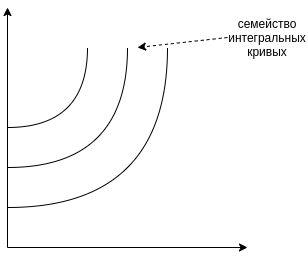
\includegraphics[width=8cm]{sem_int}}
	%\caption{График зависимости $T(x)$ при $F_0 = 0$ (шаш 0.0001).}
	\label{fig:sem_int}
\end{figure}

Для того чтобы выбрать одну кривую, необходимо начальное условие. Если ДУ n-го
порядка, нужно n НУ. 

Уравнение n-го порядка содержит n произвольных констант. Решение с этими
константами определяет общее решение ДУ. Для выделения частного решения
константы должны быть определены. Для этого задаются дополнительные условия.

Различают три основных типа задач для ОДУ: задачи Коши, краевае задачи
и задачи на собственные значения.

Если все условия ставятся в одной точке, то это задача Коши.

\begin{equation*}
	\begin{cases}
		u_k'(x) = f_k(x, u, u_1, u_2, ..., u_n), k = 1..n \\
		u_k(\xi) = \eta_k, k = 1..n
	\end{cases}
\end{equation*}

Условия $u_k(\xi) = \eta_k, k = 1..n$ можно рассматривать как задание координат 
начальной точки $(\xi, \eta_1, \eta_2, ..., \eta_n)$ интегральной кривой в 
$(n + 1)$-мерном пространстве $(x, u_1, u_2, ..., u_n)$.

Если условия ставятся в разных точках, то это краевая задача. В уравнении первого порядка
не может быть краевой задачи.

Краевая задача -- задача о нахождении решения ОДУ, 
удовлетворяющего краевым условиям в конце интервала или
на границе области.

Например, требуется найти решение краевой задачи для дифференци-
ального уравнения второго порядка

$u'' + p(x) u' + q(x) u = f(x)$

на отрезке $[a, b]$, удовлетворяющего на концах отрезка условиям:

$u(a) = A; \, \, \, \, \, \, u(b) = B$.

Здесь $A, B$ -- постоянные. Граничные условия могут быть заданы и в более
общем виде:

$\alpha_1 u(a) + \beta_1 u'(a) = A;$

$\alpha_2 u(b) + \beta_2 u'(b) = B.$

Методы решения краевых задач подразделяются на точные аналитиче-
ские, приближённые и численные.

Аналитические методы применимы лишь для решения узкого класса уравнений. 
К приближенным методам решения краевых задач относятся разложение в ряды Фурье,
методы Ритца и Галеркина. Для численного решения краевых задач применяют
метод стрельбы и разностный метод.

\textbf{8. Метод Пикара в задаче Коши для  ОДУ.  Привести пример.}

Методы решения задачи Коши для ОДУ:

\begin{itemize}
	\item точный метод;
	\item приближенный аналитический метод;
	\item численный метод.
\end{itemize}

К \textbf{точным} относятся методы, позволяющие выразить решение ДУ 
через элементарные функции, либо представить его при помощи квадратур от
элементарных функций.

Классы уравнений, для которых разработаны методы получения точных решений, сравнительно 
узки и охватывают только малую часть возникающих на практике задач.

В ряде случаев точное решение ДУ представляет из себя неявную
функцию. Тогда для получения зависимости $u$ от $x$ необходимо применять численнные
методы (метод ньютона, половинное деление).

Например, доказано, что решение уравнения $u'(x) = x^2 + u^2$ не выражается через элементарные
функции.

В приближенных методах решение получается как предел $u(x)$ некоторой
последовательности $y_n(x)$, причем $y_n(x)$ выражаются через элементарные функции
или при помощи квадратур. Ограничиваясь конечным числом n, получаем приближенное
выражение для $u(x)$.

Численные методы -- это алгоритмы вычисления приближенных значений искомого решения
$u(x)$ на некоторой выбранной сетке значений аргумента $x_n$. Численные методы
могут дать только частное решение. Зато эти методы универсальные (применимы для уравнений,
которые имеют или не имеют аналитического решения).

Приближенный аналитический метод: метод Пикара.

Метод Пикара является обобщением метода последовательных приближений.

Рассмотрим задачу Коши для уравнения первого порядка

\begin{eqnarray}
	\begin{cases}
		u'(x) = f(x, u(x)) \\
	u(\xi) = \eta.
	\end{cases}
\end{eqnarray}

Интегрируя ДУ, заменим эту задачу эквивалентным ей интегральным уравнением типа
Вольтерра

\begin{eqnarray}
	u(x) = \eta + \int\limits_{\xi}^x f(t, u(t)) d t.
\end{eqnarray}

Решая это интегральное уравнение методом последовательных приближений,
получим итерационный процесс Пикара

\begin{eqnarray}
	y_s(x) = \eta + \int\limits_{\xi}^x f(t, y_{s-1}(t)) dt; \, \, \, \, y_0(x) = \eta
\end{eqnarray}
 
(приближенное решение обозначается через $y$). На каждой итерации этого процесса
интегрирование выполняется либо точно, либо численными методами.

Метод сходится, если функция
ограничена по своим параметрам и удовлетворяет условию Липшица:

\textit{для любых двух точек $(x_1, u_1)$ и $(x_2, u_2)$:
	$\left| f(x_1, u_1) - f(x_2, u_2) \right| \leq L(|x_1 - x_2| + |u_1 - u_2|)$, 
	где $L$ -- константа Липшица.}

\textbf{Пример}

Применим метод Пикара к задаче Коши для уравнения

\begin{equation}
	\begin{cases}
		u'(x) = x^2 + u^2, \\
		u(0) = 0,
	\end{cases}
\end{equation}

решение которого не выражается через элементарные функции.

Получим

$y_0(x) = 0$

$y_1 = \frac{1}{3} x^3$

$y_2 = \frac{1}{3} x^3 \left( 1 + \frac{1}{21} x^4 \right)$

$y_3 = \frac{1}{3} x^3 \left( 1 + \frac{1}{21} x^4 + \frac{2}{693} x^8 + \frac{1}{19845} x^12 \right),$

и т.д. Видно, что при $x \leq 1$ эти приближения быстро сходятся и позволяют
вычислить решение с высокой точностью.

Метод Пикара выгодно применять, если интегралы (5) удается вычислить
через элементарные функции. Если же правая часть уравнения (3)
более сложна, так что эти интегралы приходится находить численными методами,
то метод Пикара становится не слишком удобным.

Метод Пикара легко обобщается на системы уравнений. Однако на практике 
чем выше порядок системы, тем реже удается точно вычислять 
интегралы (5), что ограничивает применение метода в этом случае.

\textbf{Метод Рунге - Кутта 2-го порядка точности в задаче Коши для  ОДУ.  Оценка точности.}

Имеем:

\begin{equation}
	\begin{cases}
		u'(x) = f(x, u(x)) \\
		u(\xi) = \eta \\
		a \leq x \leq b
	\end{cases}
\end{equation}

\begin{figure}[!h]
	\center{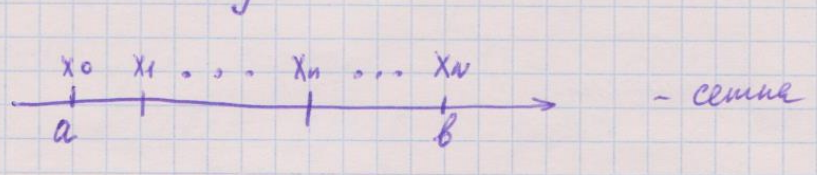
\includegraphics[width=16cm]{setka}}
	%\caption{График зависимости $T(x)$ при $F_0 = 0$ (шаш 0.0001).}
	\label{fig:setka}
\end{figure}

В области интегрирования $[a, b]$ вводится сетка. Сетка -- множество
точек на отрезке $[a, b]$ таких, что 

$W = \{ x : a = x_0 < x_1 < x_2 < ... < x_n < x_{n+2} < ... < x_N \}$

Расстояние между узлами -- шаг:

$h_n = x_n - x_{n-1}$.

Шаг может быть переменным или постоянным.

$h_n = const$

$W_n = \{ x_i : x_i = a + i h; i = 1..N \}$

Функция, полученная в результате применения численного метода на выбранной сетке
называется сеточной. 

$y_i \rightarrow u(x_i)$ при $h \rightarrow 0$.

Сеточная функция сходится в точному в точке $X$, если
$|y_i - u(x_i)| \ rightarrow 0$ при $h \rightarrow 0$. 
Сеточное решение сходится к точному на отрезке $[a, b]$, если
оно сходится в каждой точке этого отрезка.

Решение имеет p-й порядок точности, если $|y_i - u(x_i)| = O(h^p)$ при $h \rightarrow 0$. Если шаг неравномерный, то 
$|y_i - u(x_i)| = O(h_{max})$ при $h \rightarrow 0$.

Имеем:

\begin{equation}
	\begin{cases}
		u'(x) = f(x, u(x)) \\
		u(\xi) = \eta 
	\end{cases}
\end{equation}

\begin{figure}[!h]
	\center{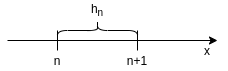
\includegraphics[width=6cm]{rk2}}
	%\caption{График зависимости $T(x)$ при $F_0 = 0$ (шаш 0.0001).}
	\label{fig:rk2}
\end{figure}

Разложения в ряд Тейлора:
\begin{eqnarray}
	u_{n+1} = u_n + \frac{h_n}{1!} u_n' + \frac{h_n^2}{2!} u_n'' + \frac{h_n^3}{3!}u_n''' + ...
\end{eqnarray}

$u_n = u(x_n)$

$u_n' = u'(x_n)$

Получим формулы второго поряжка точности метода Рунге-Кутта.

Приближенное решение обозначим через $y$.

$u_n' = f(x, u_n), \, \, \, \, \, \, u_n = u(x_n)$

\begin{eqnarray}
	y_{n+1} = y_n + h_n f(x_n, u_n) + \frac{h_n^2}{2!} u_n''
\end{eqnarray}

\begin{eqnarray}
	u_n'' = (u_n)' = \frac{df(x, u)}{dx} \bigg|_{x_n} = f'_x (x_n, y_n) + f'_y (x_n, y_n) \cdot f(x_n, y_n)
\end{eqnarray}

\begin{eqnarray}
	y_{n+1} = y_n + h_n f(x_n, y_n) + \frac{h_n^2}{2} \left[ f'_x (x_n, y_n) + f'_y (x_n, y_n) \cdot f(x_n, y_n) \right]
\end{eqnarray}

\begin{eqnarray}
	u_n' = \frac{df}{dx} = \frac{f(x_n + \gamma h_n, y_n + \delta h_n) - f(x_n, y_n)}{\Delta x}
\end{eqnarray}

Подставим (13) в (10):

\begin{eqnarray}
	y_{n+1} = y_n + h_n f(x_n, y_n) + \frac{h_n^2}{2!} \left[\frac{ f(x_n + \gamma h_n, y_n + \delta h_n) - f(x_n, y_n) }{ \Delta x }\right] = \nonumber \\
	= y_n + h_n \left[ \beta f(x_n, y_n) + \alpha f(x_n + \gamma h_n, y_n + \delta h_n) \right]
\end{eqnarray}

$\beta$ подлежит определению. Разложим $f(x_n + \gamma h_n, y_n + \delta h_n)$ 
в ряд Тейлора.

\begin{eqnarray}
	y_{n+1} = y_n + h_n \left\{ \beta f(x_n, y_n) + \alpha \left[ f(x_n, y_n) + f'_x \gamma h_n + f'_y \delta h_n \right] \right\} = \nonumber \\
	= y_n + h_n(\alpha + \beta) f(x_n, y_n) + \alpha \gamma h_n^2 f'_x + \alpha \delta f'_y h_n^2
\end{eqnarray}

Сравнивая (15) и (12) видим:

\begin{equation}
	\begin{cases}
		\alpha + \beta = 1 \\
		\alpha \gamma = \frac{1}{2} \\
		\alpha \delta = \frac{1}{2} f(x_n, y_n)
	\end{cases}
\end{equation}

\begin{equation}
	\begin{cases}
		\beta = 1 - \alpha \\
		\gamma = \frac{1}{2 \alpha} \\
		\delta = \frac{1}{2 \alpha} f(x_n, y_n)
	\end{cases}
\end{equation}

Подставим $\beta, \gamma, \delta$ в (14), получим:

\begin{eqnarray}
	y_{n+1} = y_n + h_n \left[ (1 - \alpha) f(x_n, y_n) + \alpha f(x_n + \frac{h_n}{1 \alpha}, y_n + \frac{h_n}{2 \alpha} f(x_n, y_n) ) \right]
\end{eqnarray}

(18) -- семейство однопараметрических формул Рунге-Кутта 2-го порядка точкости.

Обычно $\alpha = 1$ или $\alpha = \frac{1}{2}$.

Порядок точности: $O(max \, h^2)$. При уменьшении шага в два раза,
точность увеличивается в 4 раза.

При $\alpha = 1$:

$y_{n+1} + h_n f(x_n + \frac{h_n}{2}, y_n + \frac{h_n}{2} f(x_n, y_n))$

\newpage
\begin{figure}[!h]
	\center{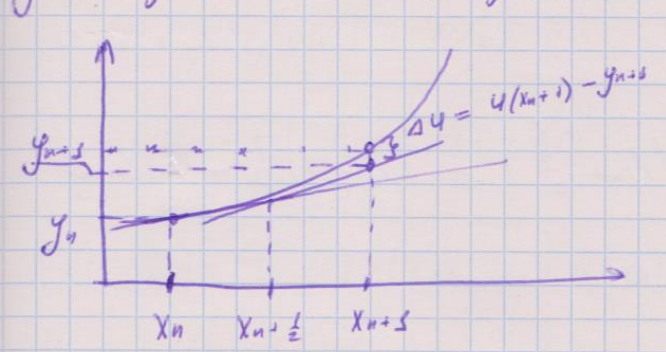
\includegraphics[width=14cm]{rk22}}
	%\caption{График зависимости $T(x)$ при $F_0 = 0$ (шаш 0.0001).}
	\label{fig:rk22}
\end{figure}

\begin{enumerate}
	\item $y_{n+1/2} = y_n + \frac{h_n}{2} f(x_n, y_n)$
	\item $y'_{n+1/2} = f(x_{n+1/2}, y_{n+1/2})$
	\item $y_{n+1} = y_n + h_n \cdot y'_{n+1/2}$
\end{enumerate}

Оценим погрешность метода.

$y_{n+1} = y_n + h \left[ (1 - \alpha) f(x_n, y_n) + \alpha f(x_n + \frac{h}{2 \alpha}, y_n + \frac{h}{2 \alpha} f(x_n, y_n) ) \right]$

$u'(x) = f(x)$

$\int\limits_{x_n}^{x_{n+1}} \frac{du}{dx} dx = \int\limits_{x_n}^{x_{n+1}} f(x) dx $

$u_{n+1} = u_n + \int\limits_{x_n}^{x_{n+1}} f(x) dx $

При $\alpha = 1$:

$y_{n+1} = y_n + h f(x_n + \frac{h}{2s})$

$R = \frac{x_N - x_0}{24} h^2 max_{x_0 \leq x \leq x_N} |f''(x)|$

При $\alpha = \frac{1}{2}$:

$y_{n+1} = y_n + \frac{h}{2} \left[ f(x_n+ + f(x_n + h) \right]$ -- метод трапеций

$R = \frac{x_N - x_0}{12} h^2 max_{x_0 \leq x \leq x_N} |f''(x)|$ -- мажорантная оценка

Численные коэффиценты в остаточных членах формулы малы;
это является одной из причин хорошей точности схем Рунге-Кутта.

Мажорантная оценка сильно завышена, больше нее погрешности не будет.

\textbf{10. Метод Рунге - Кутта 4-го порядка точности в задаче Коши для  ОДУ.  Оценка точности.}

Преимущества схем Рунге-Кутта:

\begin{itemize}
	\item явные -- для перехода из n в (n+1)-й узел требуется строго определенное фиксированное количество операций;
	\item формулы достаточно точные;
	\item формулы позволяют вести расчеты с разным (переменным) шагом.
\end{itemize}

\textbf{Метод Рунге-Кутта 4-го порядка точности}

$y_{n+1} = y_n + \frac{h_n}{6} (k_1 + 2 k_2 + 2k_3 + k_4)$

$k_1 = f(x_n, y_n)$

$k_2 = f(x_n + \frac{h_n}{2}, y_n + \frac{h_n}{2}k_1)$

$k_3 = f(x_n + \frac{h_n}{2}, y_n + \frac{h_n}{2}k_2)$

$k_4 = f(x_n + h_n, y_n + h_n k_3)$

Рассмотрим обобщение формулы на случай двух переменных. Пусть дана система

\begin{equation*}
 \begin{cases}
   u'(x) = f(x, u, v) \rightarrow y \\
   v'(x) = \varphi(x, u, v) \rightarrow z \\
   v(\xi) = v_0 \\
   u(\xi) = u_0 \\
 \end{cases}
\end{equation*}

Тогда

$y_{n+1} = y_n + \frac{k_1 + 2k_2 + 2k_3 + k_4}{6}$

$z_{n+1} = z_n + \frac{q_1 + 2q_2 + 2q_3 + q_4}{6}$

$k_1 = h_n f(x_n, y_n, z_n)$

$k_2 = h_n f(x_n + \frac{h_n}{2}, y_n + \frac{k_1}{2}, z_n + \frac{q_1}{2})$

$k_3 = h_n f(x_n + \frac{h_n}{2}, y_n + \frac{k_2}{2}, z_n + \frac{q_2}{2})$

$k_4 = h_n f(x_n + h_n, y_n + k_3, z_n + q_3)$

$q_1 = h_n \varphi(x_n, y_n, z_n)$

$q_2 = h_n \varphi(x_n + \frac{h_n}{2}, y_n + \frac{k_1}{2}, z_n + \frac{q_1}{2})$

$q_3 = h_n \varphi(x_n + \frac{h_n}{2}, y_n + \frac{k_2}{2}, z_n + \frac{q_2}{2})$

$q_4 = h_n \varphi(x_n + h_n, y_n + k_3, z_n + q_3)$

Оценим погрешность метода.

$u'(x) = f(x)$

$y_{n+1} = y_n + \frac{h}{6} \left( f(x_n) + 4 f(x_n + \frac{h}{2}) + f(x_n + h) \right)$

$R = \frac{x_N - x_0}{2880} h^4 max_{x_0 \leq x \leq x_N} |f^{iv}(x)|$

\textbf{11. Метод Адамса в задаче Коши для ОДУ.}

Будем рассматривать правую часть уравнения $f(x, u)$ не на всей
плоскости ее аргументов $x, u$, а только на определенной интегральной
кривой $u(x)$, соответствующей искомому решению. Тогда она
будет функцией только одного аргумента $x$; обозначим ее через 
$F(x) = f(x, u(x))$.

Пусть нам уже известно приближенное решение в нескольких точках
сетки $y_n, y_{n-1}, ..., y_{n-m}$. Тогда в этих точках известны также
$F(x_k) = f(x_k, y_k)$. В окрестности этих узлов можно приближено
заменить $F(x)$ интерполяционным многочленом; запишем его
для неравномерной сетки в форме Ньютона:

\begin{eqnarray}
	F(x) = F(x_n) + (x - x_n) F(x_n, x_{n-1}) + \nonumber \\
	+ (x - x_n) (x - x_{n-1})F(x_n, x_{n-1}, x_{n-2}) + \nonumber \\
	+ (x - x_n) (x - x_{n-1}) (x - x_{n-2}) F(x_n, x_{n-1}, x_{n-2}, x_{n-3}) + ...
\end{eqnarray}

Ограничимся только написанными членами, так как уже они обеспечивают
четвертый порядок точности. Для вычисления решения в следующей точке запишем
ДУ в интегральной форме

\begin{eqnarray}
	u_{n+1} = u_n + \int\limits_{x_{n}}^{x_{n+1}} f(x, u(x)) dx = u_n \int\limits_{x_{n}}^{x_{n+1}} F(x) dx
\end{eqnarray}

и подставим в него интерполяционный многочлен (19). Получим формулу
Адамса для переменного шага

\begin{eqnarray}
	y_{n+1} = y_n + h_n F(x_n) + \frac{1}{2} h_n^2 F(x_n, x_{n-1}) + \nonumber \\
	+ \frac{1}{6} h_n^2 (2h_n + 3h_{n-1}) F(x_n, x_{n-1}, x_{n-2}) + \nonumber \\
	\frac{1}{12} h_n^2 (3 h_n^2 h_{n-1} + 4 h_n h_{n-2} + 6 h_{n-1}^2 + 6 h_{n-1} h_{n-2}) \cdot \nonumber \\
	\cdot F(x_n, x_{n-1}, x_{n-2}, x_{n-3}),
\end{eqnarray}

где $h_n = x_{n_1} - x_n$.

Эта формула имеет четвертый порядок точности. Если отбросить последнее слагаемое,
получим формулу третьего порядка точности. Аналогично получаются формулы
низших порядков.

Чаще используется менее громоздкий вариант формулы (21), рассчитаный
на постоянный шаг интегрирования. Вместо разделенных разностей воспроизводят
конечные разности $\Delta^p F_n = p! F(x_n, x_{n-1}, ..., x_{n-p})$, приблизительно
равные $p$-й производной в точке $\frac{(x_n + x_{n-p})}{2}$, и получают

\begin{eqnarray}
	y_{n+1} = y_n + F_n+ \frac{1}{2} h^2 \Delta^1 F_n + \frac{5}{12} h^3 \Delta^2 F_n + \frac{3}{8} h^4 \Delta^3 F_n.
\end{eqnarray}

Остаточный член этой формулы равен $\frac{251}{750} h^5 F^{iv}(x)$

Чтобы начать расчет методом Адамса, недостаточно знать $y(x_0)$.
Для начала расчета по формуле (21) надо знать величину решения в четырех
точках $x_0, x_1, x_2, x_3$ (а при формуле p-го порядка точности -- в p точках).
Поэтому надо вычислить недостающие значения $y_n$ каким-либо другим
методом -- методом Рунге-Кутта, или разложением по формуле Тейлора с
достаточно большим числом членов. При работе на ЭВМ это увеличивает
объем программы. Кроме того, формулы (21) громоздки, а несложные формулы (22)
рассчитаны только на постоянный шаг и требуют нестандартных действий при
смене шага: надо перейти к формулам (21), сделать по ним четыре шага и снова
вернуться к формулам (22). Все это делает метод Адамса неудобным для расчетов на ЭВМ.

Метод Адамса привлекателен тем, что за один шаг приходится только один
раз высчислять $f(x, u)$, которая может быть очень сложной. А в 
четырехчленной схеме Рунге-Кутта того же порядка точности $f(x, u)$ вычисляется 
за шаг четыре раза. Однако коэффицент в остаточном члене схемы Рунге-Кутта меньше
в 960 раз, чем в (22). Значит при одинаковой точности схема Рунге-Кутта
позволяет брать шаг в 5.7 раз крупнее, то есть фактически вычислять 
$f(x, u)$ даже меньшее число раз, чем в методе Адамса.

Поэтому сейчас метод Адамса используется реже метода Рунге-Кутта.

\textbf{12. Неявные численные методы (Эйлера, трапеций,  Гира) в задаче Коши для ОДУ.}

\textbf{Метод Эйлера}

$y_{n+1} = y_n + h f(x_{n+1}, y_{n+1})$

Геометрическая интерпретация одного шага метода заключается в том, что 
решение на отрезке $[x_n, x_{n+1}]$ аппроксимируется касательной
$y = y_{n+1} + y'(x_{n+1}) (x - x_{n+1})$, проведенной в точке
$[x_{n+1}, y_{n+1}]$ к интегральной кривой, проходящей через эту точку.

\textbf{Метод трапеций}

\begin{eqnarray}
	y_{n+1} = y_n + \int\limits_{x_n}^{x_{n+1}} f(x, u(x)) dx
\end{eqnarray}

\begin{eqnarray}
	y_{n+1} = y_n + \frac{h}{2} \left[ f(x_n, y_n) + f(x_{n+1}, y_{n+1}) \right] + O(h^2)
\end{eqnarray}

Эта схема имеет второй порядок точности, допускает счет с неравномерным
шагом, не требует специальных приемов для начала счета.

Но у этой схемы есть серьезные недостатки. Во-первых, неизвестно, имеет ли уравнение (24)
вещественный корень, то есть разрешима ли задача. Можно привести пример, когда
при большом шаге корня нет. Пусть $f(x, u) = u^2$ и $u(0) = 1$;
тогда на первом шаге $y_1 =  1 + \frac{1}{2} h (1 + y_1^2)$ 
и при $h > (1 + \sqrt{2})^{-1}$ вещественного корня нет.

Во-вторых, даже если корень есть, то как его найти? Метод ньютона применять 
нежелательно, так как для этого надо дифференцировать $f(u, x)$. Метод 
деления пополам не обобщается на системы уравнений. Остается метод 
последовательных приближений 

\begin{eqnarray}
	y_{n+1}^{(s)} = y_n + \frac{1}{2} h [f(x_n, y_n) + f(x_{n+1}, y_{n+1}^{(s-1)})]
\end{eqnarray}

Однако он сходится к корню, только если $h |f_u| < 2$, то есть 
при достаточно малом шаге. Если в ходе расчета $f_u$ возрастает, то итерации
(25) могут перестать сходиться. 

От последней трудности можно избавиться, заодно уменьшив объем вычислений. Для этого 
заранее ограничивается число итераций и (25) рассматривается как самостоятельная 
явная схема.

\textbf{Методы Гира}

Методом Гира называют один из множества методов решения жестких задач Коши, основанных на 
такназываемых формулах дифференцирования назад.

Метод Гира относится к неявным многошаговым разностным методам.

$\frac{3}{2} y_{n+1} - 2 y_n + \frac{1}{2} y_{n-1} = h f(x_{n+1}, y_{n+1}) + O(h^2)$

$\frac{11}{6} y_{n+1} - 3 y_n + \frac{3}{2} y_{n-1} - \frac{1}{3} y_{n-2} = h f(x_{n+1}, y_{n+1}) + O(h^3)$

Неявные методы Гира обладают хорошими свойствами устойчивости, что 
позволяет использовать их для решения жестких систем уравнений.

Для решения неявных уравнений метода Гира обычно используется 
какой-либо итерационный метод, например, метод простой итерации. 
В качестве начального приближения $y^{(0)}$ можно взять решение, 
полученное с помощью явного метода Адамса, например, третьего порядка точности.

Благодаря относительной простоте и высокой устойчивости алгоритм приобрел большую популярность и считается 
<<промышленным стандартом>> для решения систем большой жесткости.

\textbf{13. Метод коллокаций в краевой задаче для ОДУ. Привести пример.}

Этот метод позволяет найти приближённое решение краевой задачи в
виде аналитического выражения. Пусть требуется найти решение линейного
дифференциального уравнения


\begin{eqnarray}
	u'' + p(x) u' + q(x) u = f(x)
\end{eqnarray}

на отрезке $x \in [a, b]$ при краевых условиях общего вида:

\begin{eqnarray}
	\alpha_1 u(a) + \beta_1 u'(a) = A; \nonumber \\
	\alpha_2 u(b) + \beta_2 u'(b) = B.
\end{eqnarray}

Выберем некоторую совокупность линейно независимых базисных
функций $\varphi_0(x), \varphi_1(x), ..., \varphi_n(x)$ , из которых
$\varphi_0(x)$ удовлетворяет неоднородным краевым условиям (27), а остальные функции
$\varphi_i(x), i = 1, 2, ..., n$, удовлетворяют однородным краевым условиям.

Приближённое решение краевой задачи (26), (27) ищем в виде линей-
ной комбинации базисных функций

\begin{equation*}
	y = \varphi_0(x) + \sum_{i=1}^n a_i \varphi_i(x).
\end{equation*}

Такая функция $y$ удовлетворяет краевым условиям при любых $a_i$.
Подставляя функцию $y = \varphi_0(x) + \sum_{i=1}^n a_i \varphi_i(x)$ в уравнение
(26) , получим некоторый остаточный член $\psi(x, a_1, a_2, ..., a_n)$, не равный нулю, поскольку функция 
$y$ не является точным решением уравнения (26). Однако так подобрать коэффициенты
$a_i$ практически невозможно. Поэтому ограничиваются требованием 
равенства нулю невязки в заданном множестве точек $x_1, x_2, ..., x_n$ на отрезке
$[a, b]$ -- точки коллокаций. В этих точках дифференциальное уравнение
(26) будет удовлетворяться точно. Таким образом, получается система
алгебраических уравнений:

\begin{equation}
	\begin{cases}
		\psi(x_1, a_1, a_2, ..., a_n) = 0; \\
		\psi(x_2, a_1, a_2, ..., a_n) = 0; \\
		\dots \\
		\psi(x_n, a_1, a_2, ..., a_n) = 0 \\
	\end{cases}
\end{equation}

относительно неизвестных $a_i, i = 1, 2, ..., n$. 
Число точек коллокаций должно согласовываться с количеством базисных
функций. Чем больше используется базисных функций и, соответственно, 
точек коллокаций, тем точнее получается приближённое решение.

\textbf{Пример}

\begin{figure}[!h]
	\center{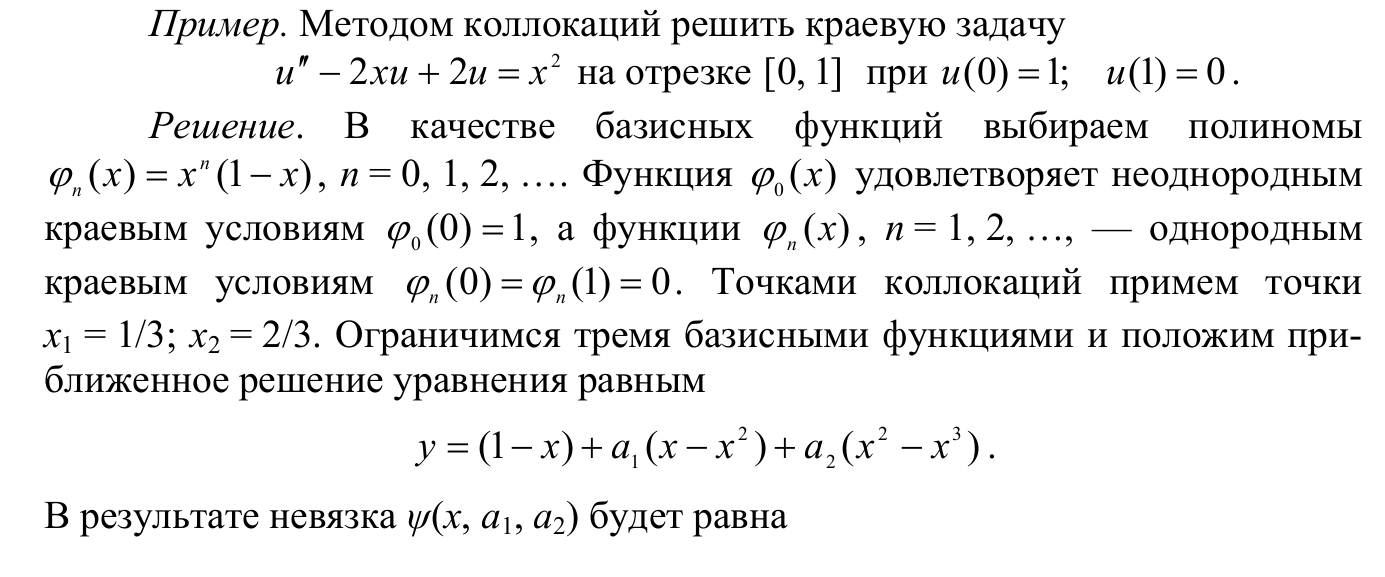
\includegraphics[width=17cm]{kollok_prim1}}
	%\caption{График зависимости $T(x)$ при $F_0 = 0$ (шаш 0.0001).}
	\label{fig:kollok_prim1}
\end{figure}

\newpage
\begin{figure}[!h]
	\center{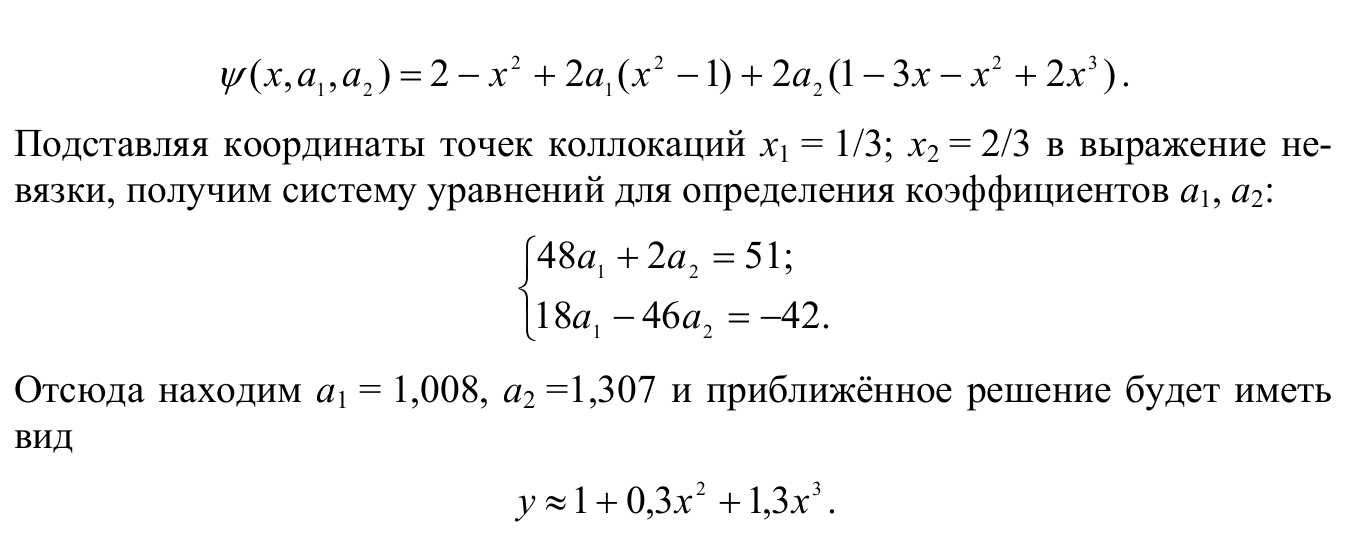
\includegraphics[width=17cm]{kollok_prim2}}
	%\caption{График зависимости $T(x)$ при $F_0 = 0$ (шаш 0.0001).}
	\label{fig:kollok_prim2}
\end{figure}

\textbf{14. Метод Галеркина в краевой задаче для ОДУ. Привести пример.}

\begin{figure}[!h]
	\center{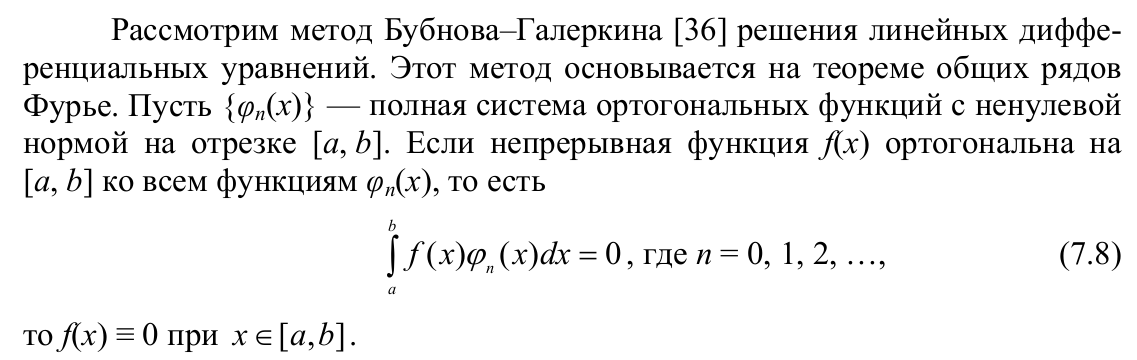
\includegraphics[width=17cm]{galerkin1}}
	%\caption{График зависимости $T(x)$ при $F_0 = 0$ (шаш 0.0001).}
	\label{fig:galerkin1}
\end{figure}
\newpage
\begin{figure}[!h]
	\center{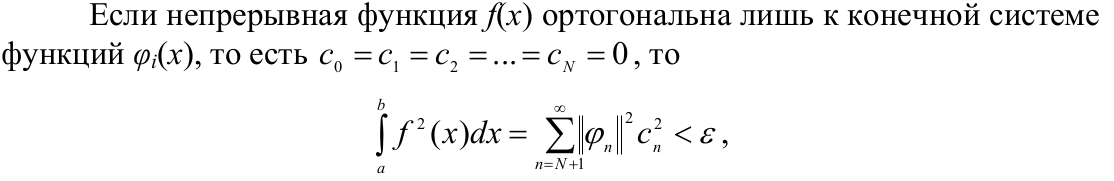
\includegraphics[width=17cm]{galerkin2}}
	%\caption{График зависимости $T(x)$ при $F_0 = 0$ (шаш 0.0001).}
	\label{fig:galerkin2}
\end{figure}

\begin{figure}[!h]
	\center{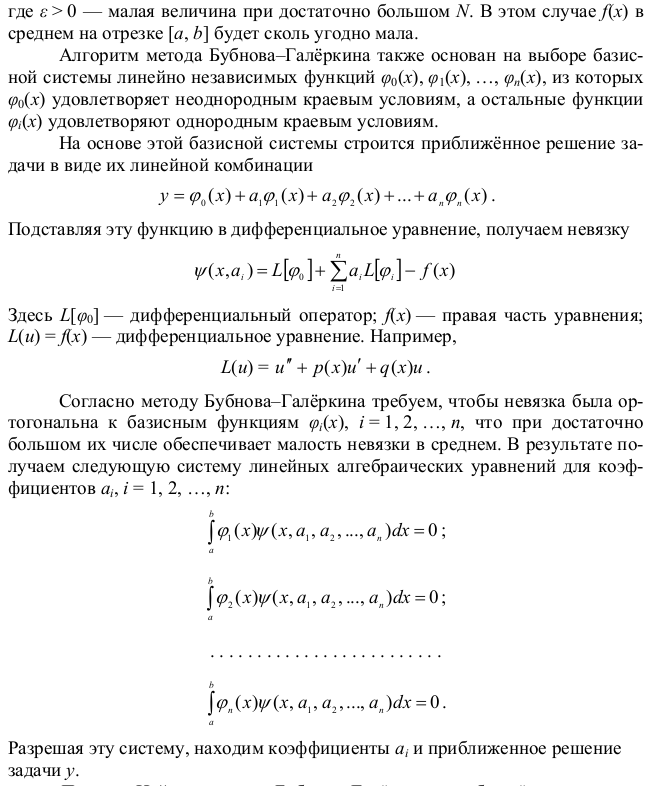
\includegraphics[width=16cm]{galerkin3}}
	%\caption{График зависимости $T(x)$ при $F_0 = 0$ (шаш 0.0001).}
	\label{fig:galerkin2}
\end{figure}

\textbf{Пример}

\begin{figure}[!h]
	\center{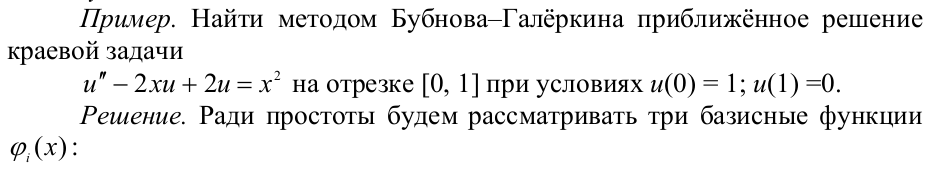
\includegraphics[width=16cm]{galerkin_pr1}}
	%\caption{График зависимости $T(x)$ при $F_0 = 0$ (шаш 0.0001).}
	\label{fig:galerkin_pr1}
\end{figure}

\begin{figure}[!h]
	\center{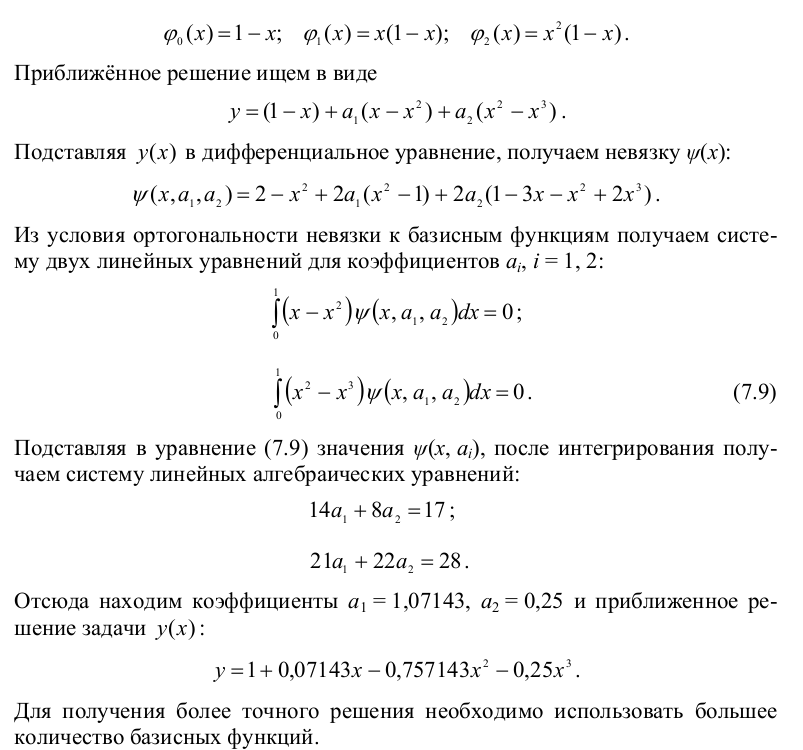
\includegraphics[width=16cm]{galerkin_pr2}}
	%\caption{График зависимости $T(x)$ при $F_0 = 0$ (шаш 0.0001).}
	\label{fig:galerkin_pr2}
\end{figure}

Метод Галеркина для нелинейных задач используют лишь для 
нахождения грубого приближения; для линейных задач
им можно найти решение с хорошей точностью. Результат очень 
чувствителен к тому, насколько удачно выбрана система функций $\varphi_k(x)$
для данной задачи.

Метод Галеркина применим только к задачам с линейным (относительно
$u(x)$ и ее производных) краевым условиям.

\newpage
\textbf{15. Сходимость разностного решения к точному на примере линейного уравнения  2-го порядка в краевой задаче для ОДУ.}

В качестве примера рассмотрим 

\begin{equation}
	\begin{cases}
		u''(x) - p(x) u(x) = f(x) \\
		u(a) = \alpha \\
		u(b) = \beta \\
		a \leq x \leq b
	\end{cases}
\end{equation}

$p(x), f(x)$ -- заданные функции.

Сводить к системе первого порядка не будем. 

Вводим сетку: 

$W_n = \left\{ x_n : x_n = a + n h, n = 0..N \right\}$

Получим простейшую разностную схему методом разностной аппроксимации.

\begin{eqnarray}
	u_n'' = \frac{u_{n-1} - 2u_n + u_{n+1}}{h^2} - \frac{1}{12} h^2 u^{iv} (\xi), \, \, \, \, \, \, x_{n-1} < \xi < x_{n+1} 
\end{eqnarray}

\begin{eqnarray}
	\frac{y_{n-1} - 2y_n + y_{n+1}}{h^2} - p_n y_n = f_n, \, \, \, \, \, \,  p_n = p(x_n), f_n = f(x_n)
\end{eqnarray}

\begin{eqnarray}
	y_{n-1} - (2 + h^2 p_n) y_n + y_{n+1} = h^2 f_n
\end{eqnarray}

Получаем систему из $N+1$ уравнений:

\begin{equation}
	\begin{cases}
		y_{n-1} - (2 + h^2 p_n) y_n + y_{n+1} = h^2 f_n \\
		y_0 = \alpha \\
		y_N = \beta.
	\end{cases}
\end{equation}

Система решается методом прогонки.

$z_n = y_n - u_n$ -- погрешность. 
Покажем, что $|z_n| \rightarrow 0$ при $h \rightarrow 0$.

Подставим в исходное уравнение уравнение второй производной:

\begin{eqnarray}
	\frac{u_{n-1} - 2u_n + u_{n-1}}{h^2} - \frac{1}{12} h^2 u^{iv}(\xi) - p_n u_n = f_n
\end{eqnarray}

\begin{eqnarray}
	u_{n-1} - (2 + h^2 p_n) u_n + u_{n+1} = \frac{1}{12} h^4 u^{iv}(\xi) + f_n h^2
\end{eqnarray}

Из (35) вычтем (32):

\begin{eqnarray}
	z_{n-1} - (2 + h^2 p_n) z_n + z_{n+1} = - \frac{1}{12} h^4 u^{iv}(\xi) \nonumber \\
	(2 + h^2 p_n)z_n = z_{n-1} + z_{n+1} + \frac{1}{12} h^4 u^{iv}(\xi) \nonumber \\
	|(2 + h^2 p_n)z_n| \leq |z_{n-1}| + |z_{n+1}| + \frac{1}{12} h^4 |u^{iv}(\xi)|
\end{eqnarray}

Возьмем m -- номер узла, где $|z_n| \rightarrow max$:

\begin{eqnarray}
	|(2 + h^2 p_n)z_m| \leq 2 |z_m| + \frac{h^4}{12} |u^{iv}(\xi)| \nonumber \\
	|z_m| \leq \frac{h^2}{12 p_n} |u^{iv}(\xi)| = O(h^2)
\end{eqnarray}

$|z_m \rightarrow 0|$ при $h \rightarrow 0$. Таким образом, разностное решение при 
$h \rightarrow 0$ сходится к точному решению. 
Разностная схема имеет 2-й порядок точности, то есть погрешность сеточной функции стремится к 0
как $O(h^2)$ при $h \rightarrow 0$.
Конструктивный способ получения решения -- метод прогонки.

\textbf{16. Получение интегро - интерполяционным методом разностной схемы для уравнения 2-го порядка с краевыми условиями 3-го рода в краевой задаче для ОДУ.}

В случае квазилинейных уравнений или в задачах с разрывными коэффициентами метод разностной аппроксимации
приводит к нарушению законов сохранения на сетке и появлению фиктивных 
источниковых слагаемых в разностном уравнении. Указанные эффекты устраняются, 
если применить так называемый интегро-интерполяционный метод получения
разностной схемы.
\newpage
\begin{figure}[!h]
	\center{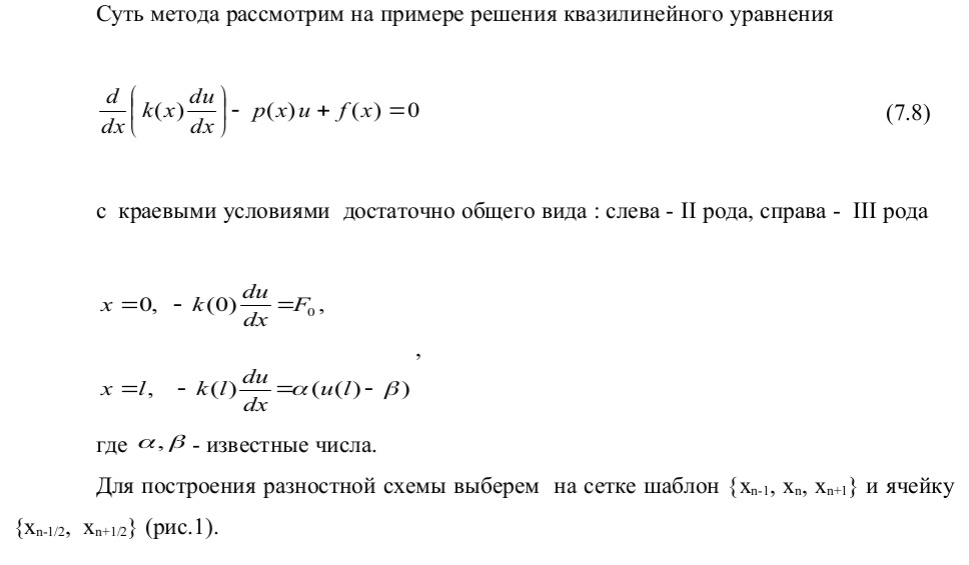
\includegraphics[width=17cm]{integr_interp}}
	%\caption{График зависимости $T(x)$ при $F_0 = 0$ (шаш 0.0001).}
	\label{fig:integr_interp}
\end{figure}
\newpage
\begin{figure}[!h]
	\center{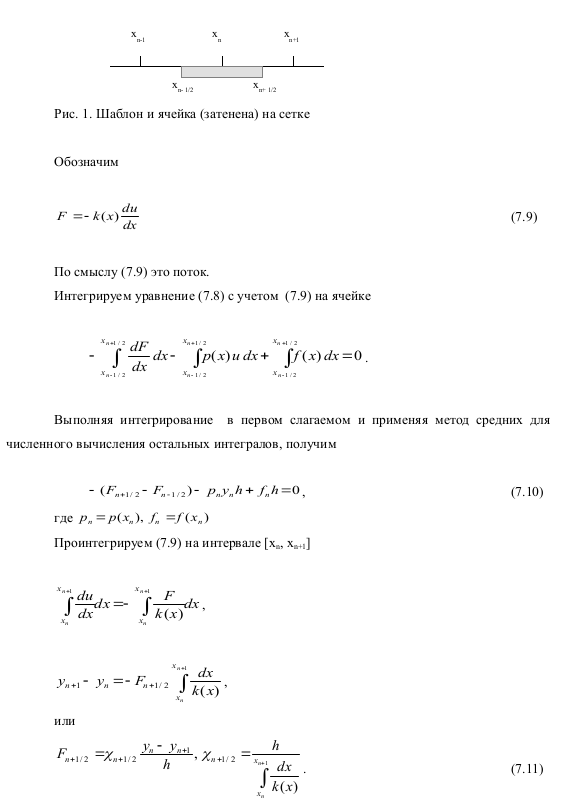
\includegraphics[width=17cm]{integr_interp2}}
	%\caption{График зависимости $T(x)$ при $F_0 = 0$ (шаш 0.0001).}
	\label{fig:integr_interp2}
\end{figure}
\newpage
\begin{figure}[!h]
	\center{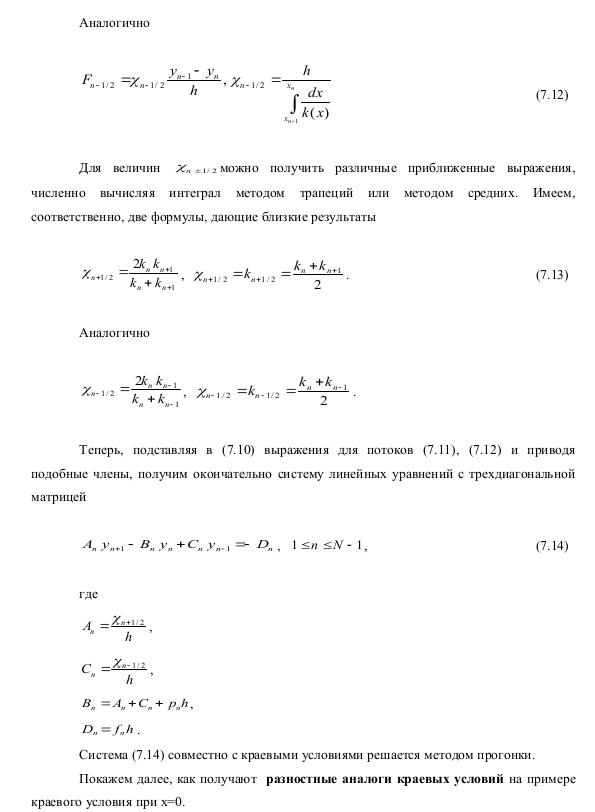
\includegraphics[width=17cm]{integr_interp3}}
	%\caption{График зависимости $T(x)$ при $F_0 = 0$ (шаш 0.0001).}
	\label{fig:integr_interp3}
\end{figure}
\newpage
\begin{figure}[!h]
	\center{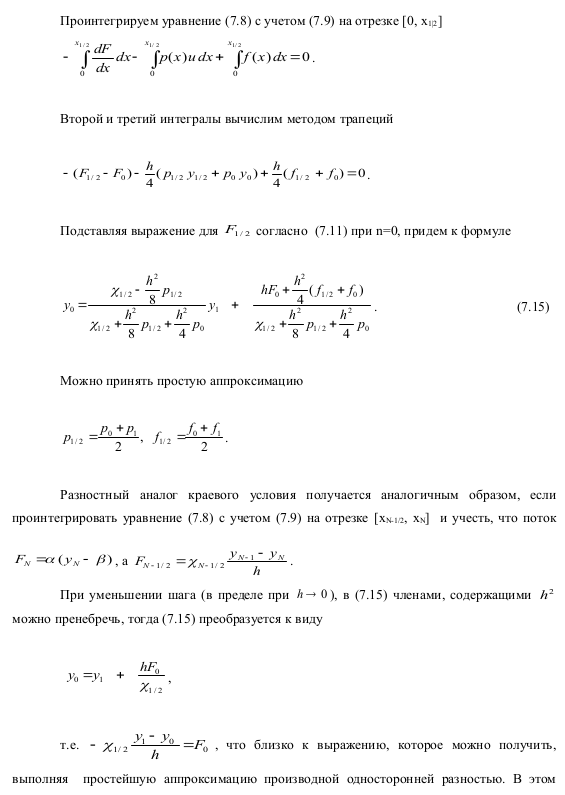
\includegraphics[width=17cm]{integr_interp4}}
	%\caption{График зависимости $T(x)$ при $F_0 = 0$ (шаш 0.0001).}
	\label{fig:integr_interp4}
\end{figure}
\newpage
\begin{figure}[!h]
	\center{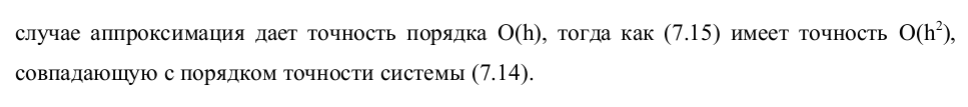
\includegraphics[width=17cm]{integr_interp5}}
	%\caption{График зависимости $T(x)$ при $F_0 = 0$ (шаш 0.0001).}
	\label{fig:integr_interp5}
\end{figure}

\textbf{17. Разностная схема для уравнения 2-го порядка с краевыми условиями 3-го рода в цилиндрических координатах в краевой задаче для ОДУ.}

см. лекция 14 с.6 или github

\textbf{18. Метод прогонки для реализации разностных схем с краевыми условиями 3-го рода.}

\textbf{19. Методы решения квазилинейных разностных схем для уравнений 2-го порядка в краевой задаче для ОДУ (простые итерации и линеаризация по Ньютону).}
\newpage
\begin{figure}[!h]
	\center{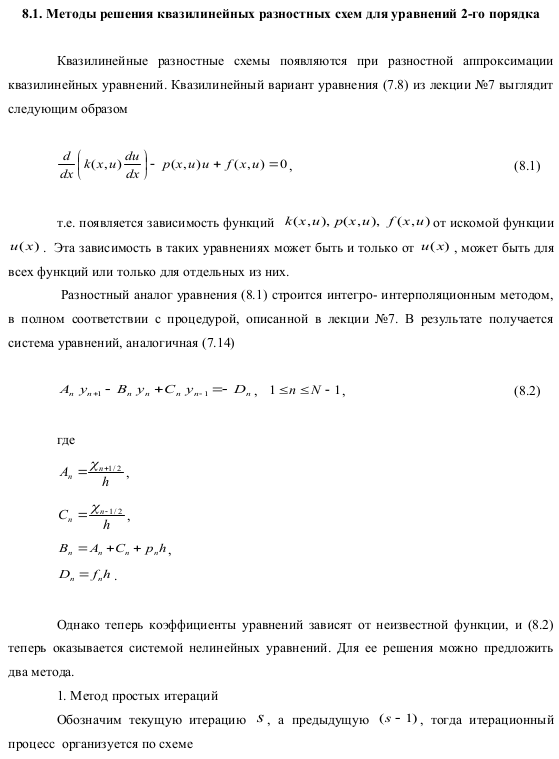
\includegraphics[width=17cm]{t191}}
	%\caption{График зависимости $T(x)$ при $F_0 = 0$ (шаш 0.0001).}
	\label{fig:t191}
\end{figure}
\newpage
\begin{figure}[!h]
	\center{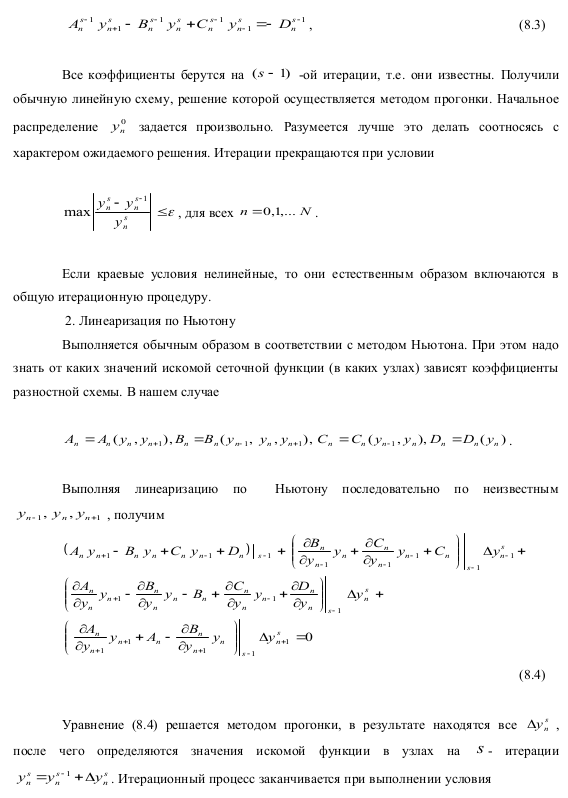
\includegraphics[width=17cm]{t192}}
	%\caption{График зависимости $T(x)$ при $F_0 = 0$ (шаш 0.0001).}
	\label{fig:t192}
\end{figure}
\newpage
\begin{figure}[!h]
	\center{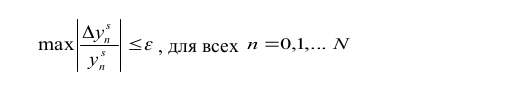
\includegraphics[width=17cm]{t193}}
	%\caption{График зависимости $T(x)$ при $F_0 = 0$ (шаш 0.0001).}
	\label{fig:t193}
\end{figure}


\textbf{20. Методы повышения порядка точности разностной аппроксимации краевых условий 2-го и 3-его рода в краевой задаче для ОДУ (разложение в ряды Тейлора и интегро- интерполяционный метод).}
\newpage
\begin{figure}[!h]
	\center{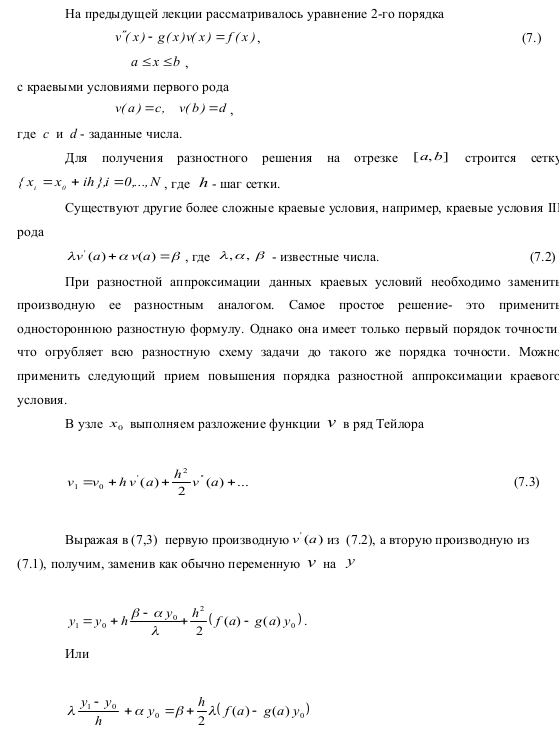
\includegraphics[width=16cm]{t201}}
	%\caption{График зависимости $T(x)$ при $F_0 = 0$ (шаш 0.0001).}
	\label{fig:t201}
\end{figure}
\newpage
\begin{figure}[!h]
	\center{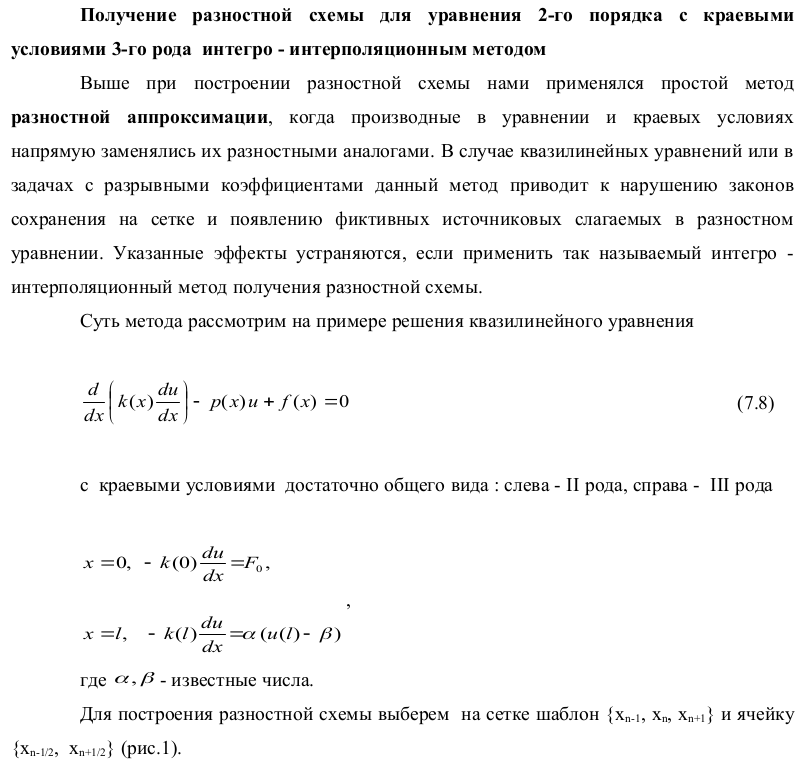
\includegraphics[width=16cm]{t202}}
	%\caption{График зависимости $T(x)$ при $F_0 = 0$ (шаш 0.0001).}
	\label{fig:t202}
\end{figure}
\newpage
\begin{figure}[!h]
	\center{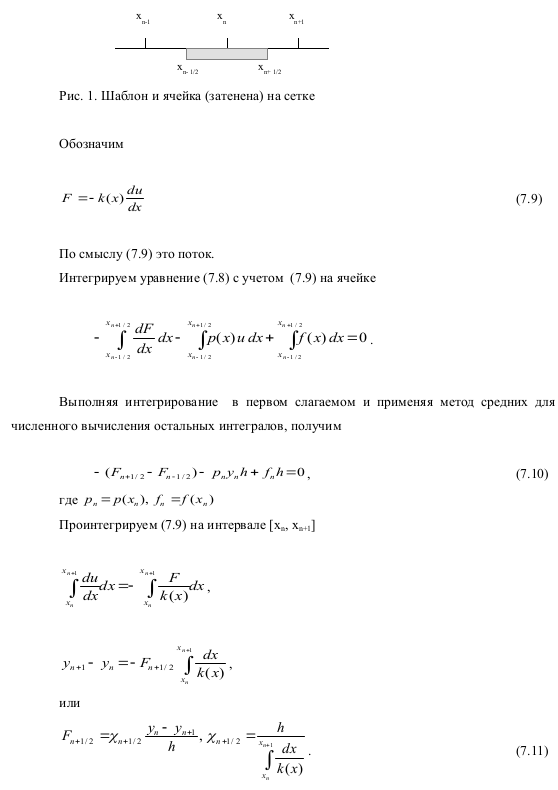
\includegraphics[width=16cm]{t203}}
	%\caption{График зависимости $T(x)$ при $F_0 = 0$ (шаш 0.0001).}
	\label{fig:t203}
\end{figure}
\newpage
\begin{figure}[!h]
	\center{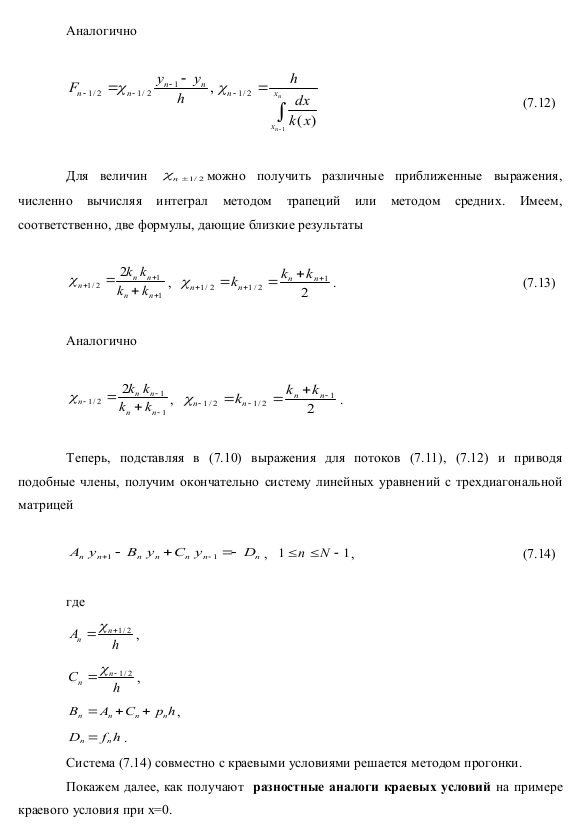
\includegraphics[width=16cm]{t204}}
	%\caption{График зависимости $T(x)$ при $F_0 = 0$ (шаш 0.0001).}
	\label{fig:t204}
\end{figure}
\newpage
\begin{figure}[!h]
	\center{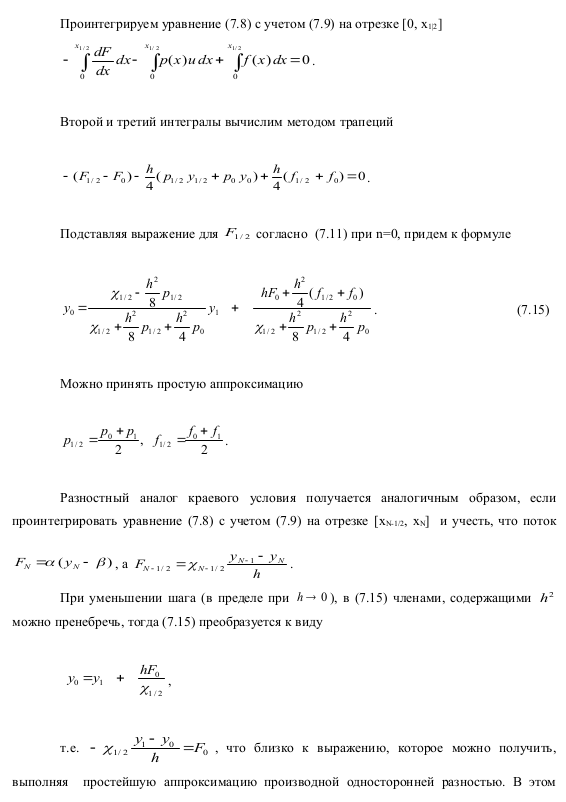
\includegraphics[width=16cm]{t205}}
	%\caption{График зависимости $T(x)$ при $F_0 = 0$ (шаш 0.0001).}
	\label{fig:t205}
\end{figure}
\newpage
\begin{figure}[!h]
	\center{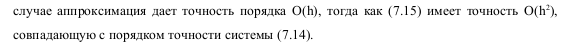
\includegraphics[width=16cm]{t206}}
	%\caption{График зависимости $T(x)$ при $F_0 = 0$ (шаш 0.0001).}
	\label{fig:t206}
\end{figure}

\textbf{21. Уравнения в частных производных. Области применения. Классификация уравнений второго порядка. Общие понятия о методах решения.}

Математические модели, построенные на основе уравнений в частных
производных, позволяют описывать поля разнообразной физической природы. Это могут
быть поля температур, плотностей, скоростей и концентраций частиц, гравитационные,
электромагнитные, радиационные поля и др. С уравнениями в частных производных
приходится иметь дело в различных областях науки и техники при формировании
моделей гидро- и газодинамики, переноса излучения, квантовой механики,
теплопередачи, физики плазмы и т. д. В указанных уравнениях в качестве независимых
переменных обычно выступают время и пространственные координаты, но могут
использоваться и такие переменные, как проекции скоростей частиц на координатные оси,
что может увеличить размерность уравнений до семи.

\newpage
\begin{figure}[!h]
	\center{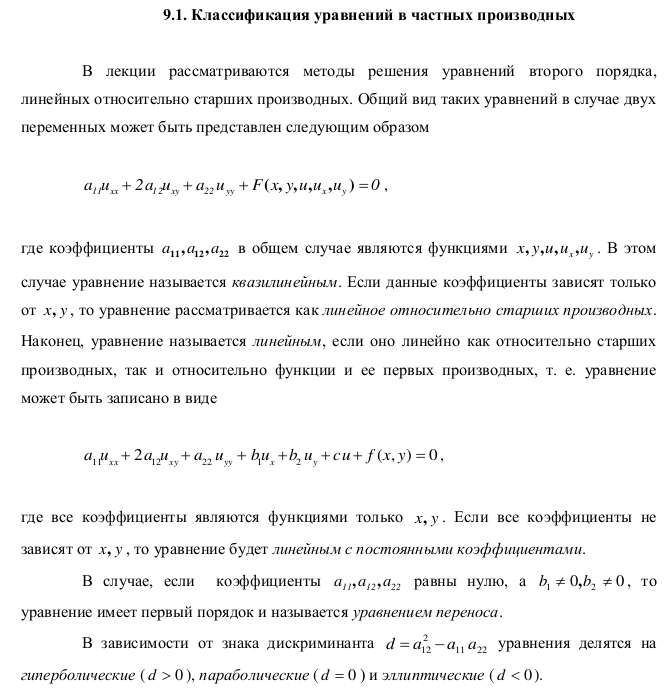
\includegraphics[width=16cm]{t211}}
	%\caption{График зависимости $T(x)$ при $F_0 = 0$ (шаш 0.0001).}
	\label{fig:t211}
\end{figure}
\newpage
\begin{figure}[!h]
	\center{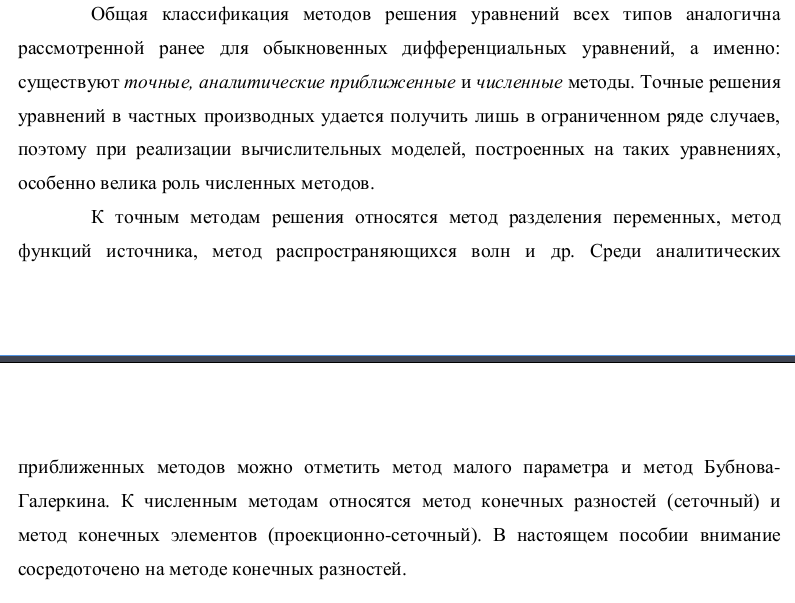
\includegraphics[width=16cm]{t212}}
	%\caption{График зависимости $T(x)$ при $F_0 = 0$ (шаш 0.0001).}
	\label{fig:t212}
\end{figure}

\textbf{22. Постановка задач Коши, краевых  и смешанных краевых задач для уравнений в частных производных. Привести примеры с краевыми условиями 1-го, 2-го и 3-го родов.}
\newpage
\begin{figure}[!h]
	\center{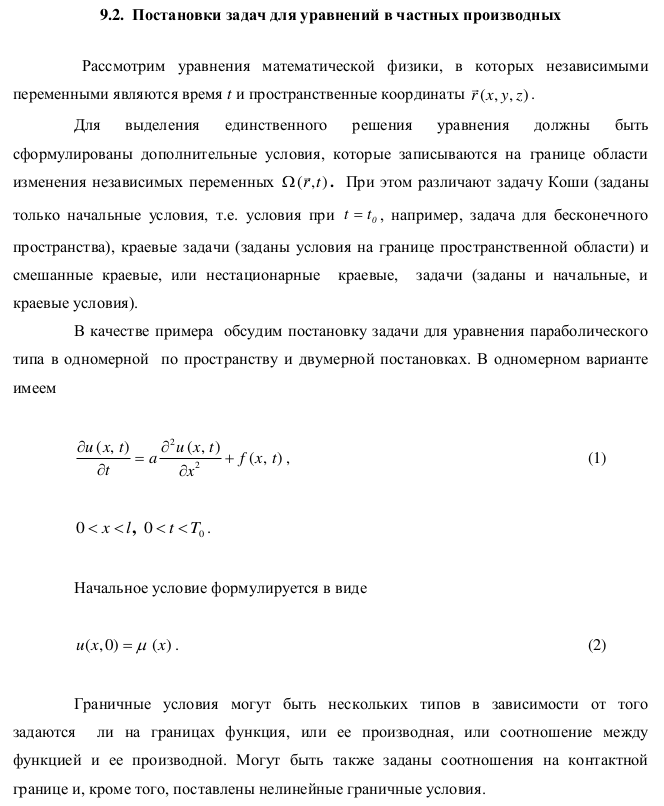
\includegraphics[width=16cm]{t221}}
	%\caption{График зависимости $T(x)$ при $F_0 = 0$ (шаш 0.0001).}
	\label{fig:t221}
\end{figure}
\newpage
\begin{figure}[!h]
	\center{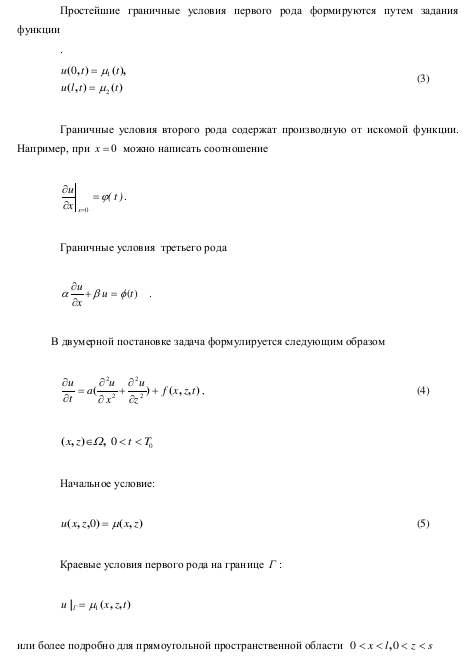
\includegraphics[width=16cm]{t222}}
	%\caption{График зависимости $T(x)$ при $F_0 = 0$ (шаш 0.0001).}
	\label{fig:t222}
\end{figure}
\newpage
\begin{figure}[!h]
	\center{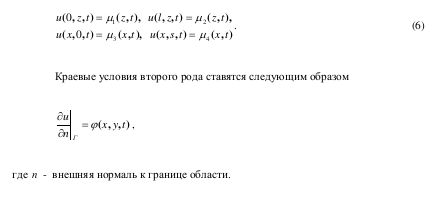
\includegraphics[width=16cm]{t223}}
	%\caption{График зависимости $T(x)$ при $F_0 = 0$ (шаш 0.0001).}
	\label{fig:t223}
\end{figure}

\textbf{23. Основные понятия метода конечных разностей на примере уравнения в частных производных с постоянными коэффициентами. Понятие о явных и неявных схемах.}
\newpage
\begin{figure}[!h]
	\center{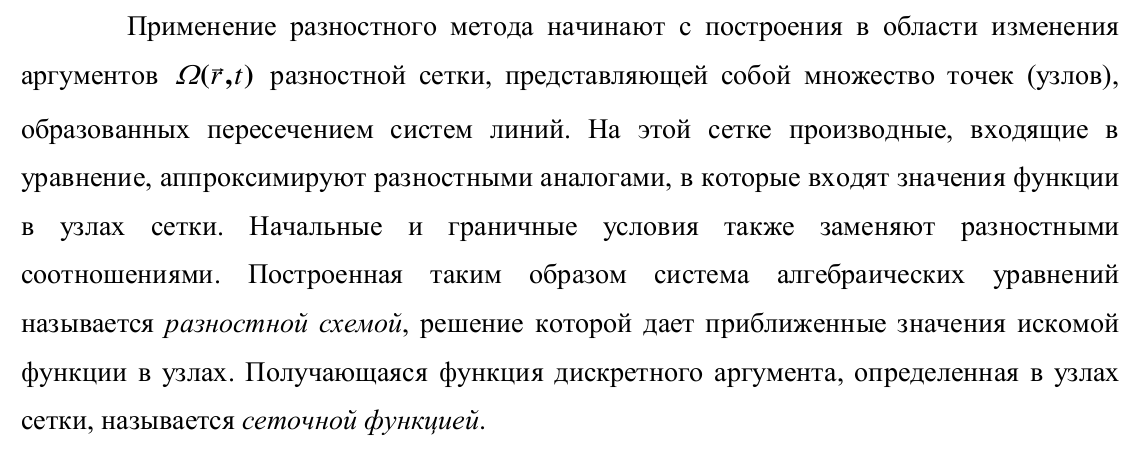
\includegraphics[width=16cm]{t231}}
	%\caption{График зависимости $T(x)$ при $F_0 = 0$ (шаш 0.0001).}
	\label{fig:t231}
\end{figure}

Рассмотрим построение сетки на примере разностной аппроксимации уравнения

\begin{figure}[!h]
	\center{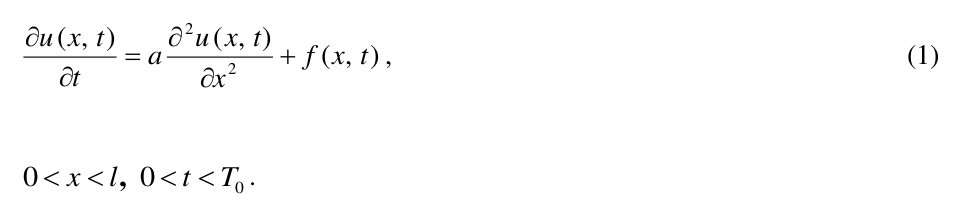
\includegraphics[width=16cm]{t232}}
	%\caption{График зависимости $T(x)$ при $F_0 = 0$ (шаш 0.0001).}
	\label{fig:t232}
\end{figure}

с дополнительными условиями

\begin{figure}[!h]
	\center{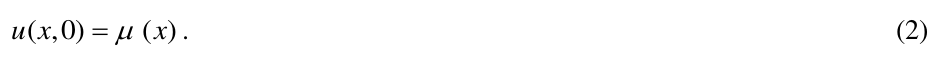
\includegraphics[width=16cm]{t233}}
	%\caption{График зависимости $T(x)$ при $F_0 = 0$ (шаш 0.0001).}
	\label{fig:t233}
\end{figure}

\begin{figure}[!h]
	\center{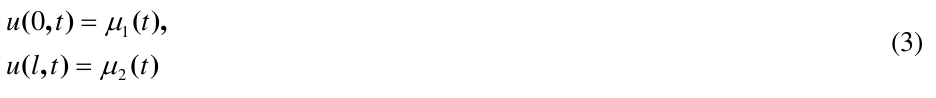
\includegraphics[width=16cm]{t234}}
	%\caption{График зависимости $T(x)$ при $F_0 = 0$ (шаш 0.0001).}
	\label{fig:t234}
\end{figure}

Построим в области интегрирования уравнения прямоугольную сетку. Последняя
образуется пересечением линий $\left\{ x_n = nh, 0 \leq n \leq N, t_m = m\tau, 0 \leq m \leq M \right\}$,
где $h, \tau$ шаги сетки по переменным $x$ и $t$. Значения функции в узлах
сетки обозначают как $u_n^m = u(x_n, t_m)$ - (рис.1.1), и, соответственно
$u_n^{m+1} = u(x_n, t_{m+1})$. Значения сеточной функции в узлах, являющейся результатом решения разностных
уравнений, обозначим $y_n^m$ и $y_n^{m+1}$, причем для удобства записи формул освободим верхний
индекс, приняв $y_n = y_n^m$ и $\hat{y}_n = y_n^{m+1}$.

\begin{figure}[!h]
	\center{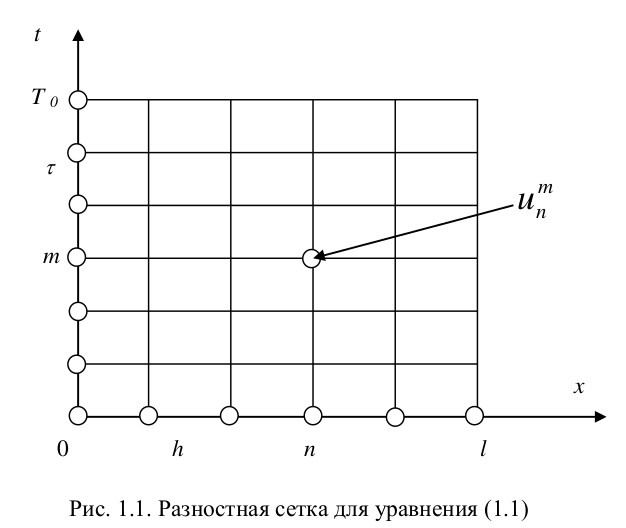
\includegraphics[width=12cm]{t235}}
	%\caption{График зависимости $T(x)$ при $F_0 = 0$ (шаш 0.0001).}
	\label{fig:t235}
\end{figure}
\newpage
Для уравнения (1.1) совокупность узлов, лежащих на линии $t=t_m$ (или на 
плоскости, если решается двумерная по пространству задача, или же на
гиперплоскости в случае многомерной постановки), называется слоем. Линии на слое,
вдоль которых меняется только одна пространственная переменная, называются
направлением. Выберем конфигурацию узлов, на которой будем проводить
аппроксимацию дифференциального уравнения. Эта конфигурация узлов называется
шаблоном. Для одной и той же задачи можно выбрать много разных шаблонов. На рис.1.2
показаны три шаблона.
\newpage
\begin{figure}[!h]
	\center{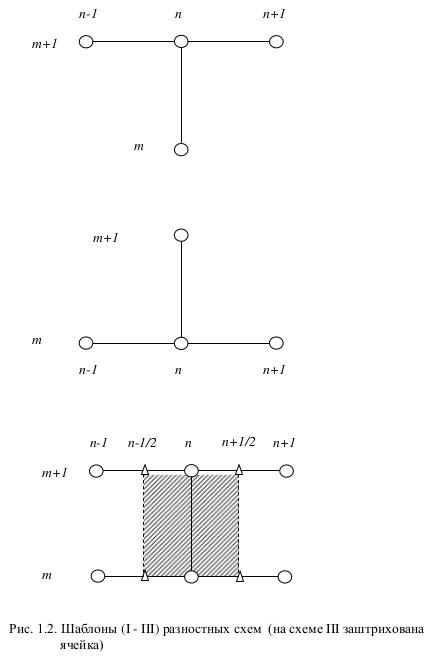
\includegraphics[width=12cm]{t236}}
	%\caption{График зависимости $T(x)$ при $F_0 = 0$ (шаш 0.0001).}
	\label{fig:t236}
\end{figure}

Заменяя в уравнении (1) производные разностными аналогами, получаем на
выбранных шаблонах соответствующие разностные схемы:

\newpage
\begin{figure}[!h]
	\center{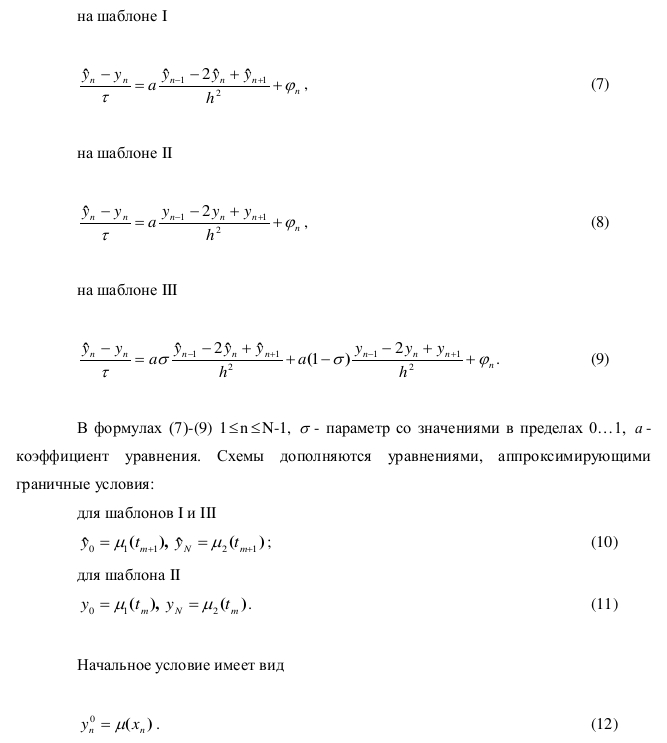
\includegraphics[width=16cm]{t237}}
	%\caption{График зависимости $T(x)$ при $F_0 = 0$ (шаш 0.0001).}
	\label{fig:t237}
\end{figure}

\newpage
\begin{figure}[!h]
	\center{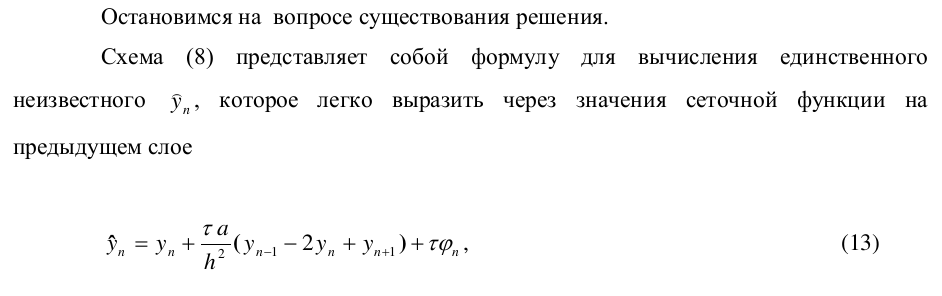
\includegraphics[width=16cm]{t238}}
	%\caption{График зависимости $T(x)$ при $F_0 = 0$ (шаш 0.0001).}
	\label{fig:t238}
\end{figure}

\newpage
\begin{figure}[!h]
	\center{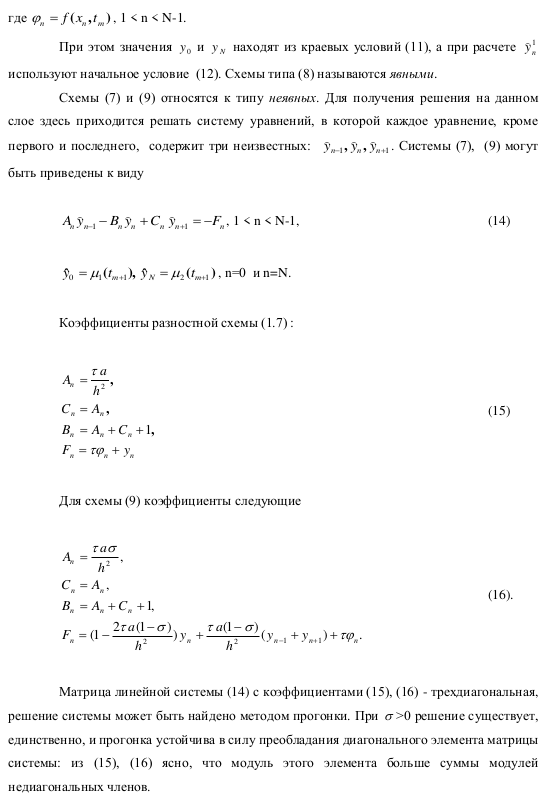
\includegraphics[width=16cm]{t239}}
	%\caption{График зависимости $T(x)$ при $F_0 = 0$ (шаш 0.0001).}
	\label{fig:t239}
\end{figure}

\newpage
\begin{figure}[!h]
	\center{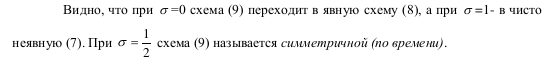
\includegraphics[width=16cm]{t2310}}
	%\caption{График зависимости $T(x)$ при $F_0 = 0$ (шаш 0.0001).}
	\label{fig:t2310}
\end{figure}

\textbf{24. Получение разностной схемы для одномерного квазилинейного параболического уравнения с краевыми условиями 3-го рода интегро-интерполяционным методом.}

см. лекцию 14 (начало)

\textbf{25. Решение разностных схем для квазилинейных уравнений в частных производных- методом простых итераций и методом  Ньютона.}

см. лекцию 8 (начало)

\textbf{26. Методы повышения порядка разностной аппроксимации  краевых условий 2-го и 3-го родов (интегро- интерполяционная процедура, разложение в ряд Тейлора) для уравнений в частных производных.}


\textbf{27. Понятие невязки для разностных схем. Привести пример вычисления невязки для неявной схемы.  Свойство аппроксимации разностных схем для уравнений в частных производных.}

Введем понятие невязки разностной схемы, построенной для дифференциального
уравнения, записанного в общем операторном виде

\begin{equation}
	Au(x) = f
\end{equation}

с дополнительными условиями

\begin{equation}
	Bu(x) = \mu(x)
\end{equation}

Разностная схема для задачи (38), (39):

\begin{eqnarray}
	A_h y = \varphi_h \\
	B_h y = \beta_h
\end{eqnarray}

Если подставить в соотношения (40) точное решение, то данное равенство будет
нарушено, так как приближенное решение $y$ не совпадает с точным решением $u$.

\textbf{Невязкой} называется величина

\begin{equation}
	\psi = \varphi_h - A_h u = (Au - f) - (A_h u -\varphi_h)
\end{equation}

Для граничных условий получаем невязку в виде

\begin{equation}
	\rho = \beta_h - B_h u = (Bu - \mu) - (B_h u - \beta_h)
\end{equation}

Дадим определение аппроксимации. Разностная схема (40), (41) аппроксимирует 
задачу (38), (39), если в некоторой норме $\| \psi \| \rightarrow 0, \| \rho \| \rightarrow 0$ 
при $h \rightarrow0$, и аппроксимация имеет p-ый порядок, если
$\| \psi \| = O(h^p),  \| \rho \| = O(h^p)$ при $h \rightarrow0$.

\begin{figure}[!h]
	\center{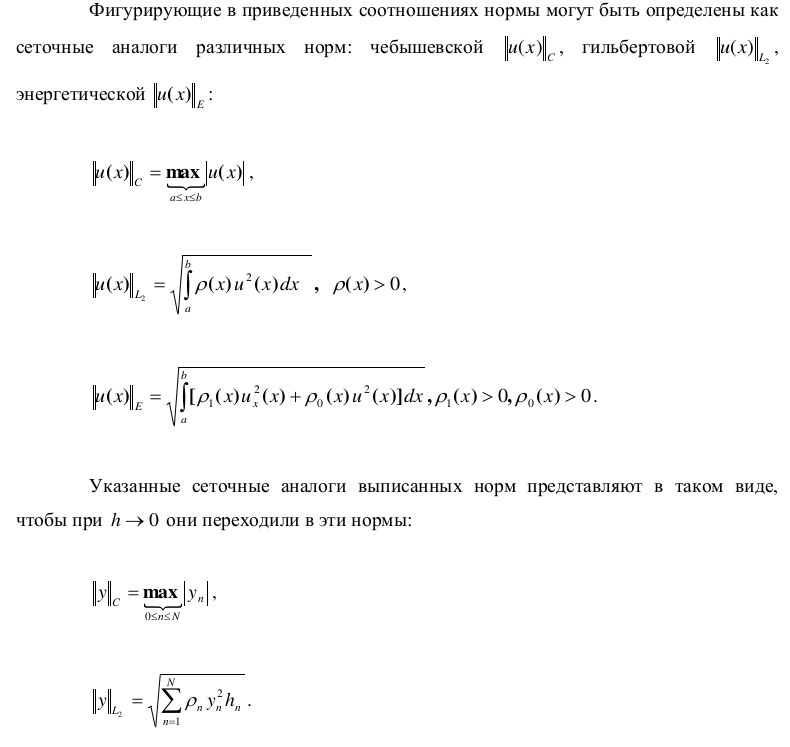
\includegraphics[width=16cm]{t271}}
	%\caption{График зависимости $T(x)$ при $F_0 = 0$ (шаш 0.0001).}
	\label{fig:t271}
\end{figure}

Невязку оценивают, проводя разложение точного решения в ряд Тейлора. Найдем
невязку разностной схемы (9) для уравнения (1).
\newpage
\begin{figure}[!h]
	\center{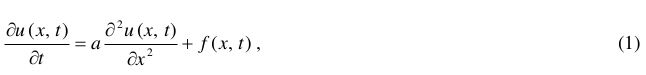
\includegraphics[width=16cm]{t272}}
	%\caption{График зависимости $T(x)$ при $F_0 = 0$ (шаш 0.0001).}
	\label{fig:t272}
\end{figure}

\begin{figure}[!h]
	\center{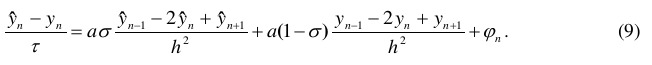
\includegraphics[width=16cm]{t273}}
	%\caption{График зависимости $T(x)$ при $F_0 = 0$ (шаш 0.0001).}
	\label{fig:t273}
\end{figure}
\newpage
\begin{figure}[!h]
	\center{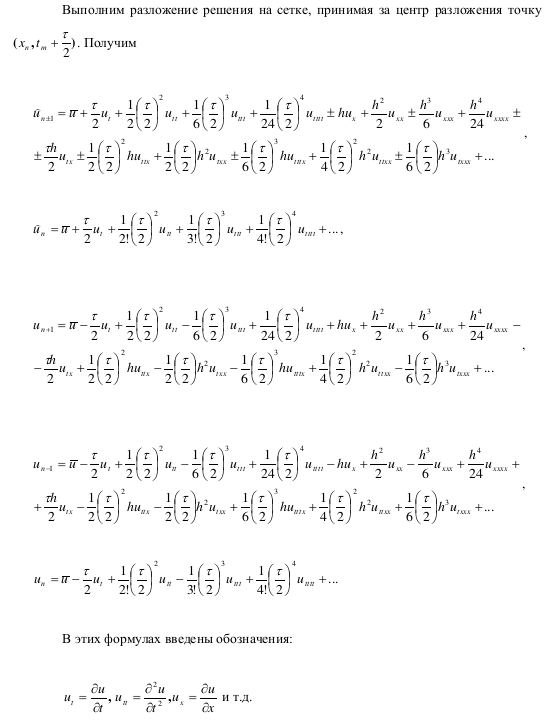
\includegraphics[width=16cm]{t274}}
	%\caption{График зависимости $T(x)$ при $F_0 = 0$ (шаш 0.0001).}
	\label{fig:t274}
\end{figure}
\newpage
\begin{figure}[!h]
	\center{\includegraphics[width=16cm]{t275}}
	%\caption{График зависимости $T(x)$ при $F_0 = 0$ (шаш 0.0001).}
	\label{fig:t275}
\end{figure}

\textbf{28. Понятие устойчивости разностных схем по начальным данным и правой части. На основе принципа максимума исследовать устойчивость явной и неявной схем для уравнения параболического типа.}

\begin{figure}[!h]
	\center{\includegraphics[width=16cm]{t281}}
	%\caption{График зависимости $T(x)$ при $F_0 = 0$ (шаш 0.0001).}
	\label{fig:t281}
\end{figure}
\newpage
\begin{figure}[!h]
	\center{\includegraphics[width=16cm]{t282}}
	%\caption{График зависимости $T(x)$ при $F_0 = 0$ (шаш 0.0001).}
	\label{fig:t282}
\end{figure}

\begin{figure}[!h]
	\center{\includegraphics[width=16cm]{t283}}
	%\caption{График зависимости $T(x)$ при $F_0 = 0$ (шаш 0.0001).}
	\label{fig:t283}
\end{figure}

см. лекция 12.

\textbf{29. На основе метода разделения переменных исследовать устойчивость четырехточечной явной разностной схемы для уравнения параболического типа.}

\textbf{30. На основе метода разделения переменных исследовать устойчивость четырехточечной неявной разностной схемы для уравнения параболического типа.}

калиткин 368

\textbf{31. На основе метода разделения переменных исследовать устойчивость шеститочечной разностной схемы для уравнения параболического типа.}

калиткин 370

\textbf{32. Сходимость разностных схем для уравнений в частных производных. Теорема о сходимости разностного решения к точному.}

см. лекция 12 с 22

\textbf{33. Продольно-поперечная схема для решения многомерных уравнений в частных производных.}

калиткин с. 391

\textbf{34. Локально-одномерный метод для решения многомерных уравнений в частных производных.}

калиткин с. 394

\textbf{Билет 16}

\textbf{1. Опишите свойство аппроксимации разностных схем для уравнений в частных производных.
Что определеяет аппроксимация, и как она соотносится со сходимостью разностного решения к точному.}

\textbf{2. Опишите алгоритм численного решения задачи Коши для ОДУ неявным методом трапеций на сетке} 
$W_n = \left\{ x_n : x_n = nh, n = 0..N \right\}$

$u^{iv} = f(x, u, u')$

$u(0) = \alpha$

$u'(0) = \beta$

$u''(0) = \gamma$

$u'''(0) = \chi$

Введем понятие невязки разностной схемы, построенной для дифференциального
уравнения, записанного в общем операторном виде

\begin{equation}
	Au(x) = f
\end{equation}

с дополнительными условиями

\begin{equation}
	Bu(x) = \mu(x)
\end{equation}

Разностная схема для задачи (44), (45):

\begin{eqnarray}
	A_h y = \varphi_h \\
	B_h y = \beta_h
\end{eqnarray}

\textbf{Невязкой} называется величина

\begin{equation}
	\psi = \varphi_h - A_h u = (Au - f) - (A_h u -\varphi_h)
\end{equation}

Для граничных условий получаем невязку в виде

\begin{equation}
	\rho = \beta_h - B_h u = (Bu - \mu) - (B_h u - \beta_h)
\end{equation}

Разностная схема (46), (47) аппроксимирует 
задачу (38), (39), если в некоторой норме $\| \psi \| \rightarrow 0, \| \rho \| \rightarrow 0$ 
при $h \rightarrow0$, и аппроксимация имеет p-ый порядок, если
$\| \psi \| = O(h^p),  \| \rho \| = O(h^p)$ при $h \rightarrow0$.

Из аппроксимации и устойчивости
следует сходимость.

Порядок точности разностного метода совпадает с порядком его аппроксимации.

\end{document}